\documentclass[a4paper,10pt,oneside,final]{article}
%\documentclass[12pt,a4paper,english]{tutthesis}
%\documentclass[11pt,final]{tutdrthesis}
%\documentclass[11pt,final]{IEEETran}

% Otetaan tarvittavat paketit mukaan 
\usepackage[dvips]{graphicx} 
\usepackage{enumerate}
\usepackage[UKenglish]{babel}
\usepackage{cite}
\usepackage{subfigure}

% 'pslatex' is otherwise equal to 'times'
% but courier font is narrower
\usepackage{pslatex}
%\usepackage{times}

% 2 pkgs for Scandinavian alphabets
\usepackage[T1]{fontenc}
\usepackage[latin1]{inputenc}

\usepackage{listings}
\usepackage{color}
\definecolor{gray95}{gray}{.95}



\lstdefinestyle{ccc} 
{ 
numbers=none, 
basicstyle=\small\ttfamily, 
keywordstyle=\bf\color[rgb]{0,0,0}, 
%commentstyle=\color[rgb]{0.133,0.545,0.133}, 
stringstyle=\color[rgb]{0.627,0.126,0.941}, 
backgroundcolor=\color{white}, 
frame=tb, %frame= lrtb, 
framerule=0.5pt, 
linewidth=\textwidth,
%aboveskip=-4.0pt,
%belowskip=-4.0pt,
lineskip=-5.0pt,
}


% style for transgen xml listings 
\lstdefinestyle{a1listing} 
{ 
numbers=none,
language=bash,
basicstyle=\small\bf\ttfamily,
emphstyle=\color[rgb]{0.0, 0.7, 0.3},
keywordstyle=\color[rgb]{0.0, 0.0, 1.0},
commentstyle=\color[rgb]{0.8, 0.0, 0.0},
stringstyle=\color[rgb]{0.737, 0.560, 0.560},
backgroundcolor=\color{gray95}, 
frame= lrtb, 
framerule=0.5pt, 
linewidth=\textwidth, 
}

% console listings style
\lstdefinestyle{console} 
{ 
numbers=none, 
basicstyle=\small\bf\ttfamily, 
backgroundcolor=\color{gray95}, 
frame=lrtb, 
framerule=0.5pt, 
linewidth=\textwidth, 
}




% 2 Completely strange definitions
\newcommand{\longpage}{\enlargethispage*{100cm} \pagebreak}
\newcommand{\nohyphens}{\hyphenpenalty=10000\exhyphenpenalty=10000\relax}


% Poikkeukselliset tavutusmuodot, erotettu v�lily�nneill�
\hyphenation{Sal-mi-nen Kan-gas Rii-hi-m�-ki Kuu-si-lin-na
  H�-m�-l�i-nen Kuk-ka-la HIBI TUTMAC Koski}
% \hyphenation{de-vel-oped pro-vides multi-stage Rctrl}

% Koitetaan estaa kuvien sijoittelu sivulle yksinaan ilman tekstia
% http://dcwww.camd.dtu.dk/~schiotz/comp/LatexTips/LatexTips.html
% Be careful not to make \floatpagefraction larger than \topfraction
\renewcommand{\topfraction}{0.85}
\renewcommand{\textfraction}{0.1}
\renewcommand{\floatpagefraction}{0.75}


%
% Define author(s) and  component's name
%
\def\defauthor{Salminen, H�m�l�inen}
\def\deftitle{HIBI v.3 \\Reference Manual}

\author{\defauthor}
\title{\deftitle}

\usepackage{fancyhdr} 
\pagestyle{fancy} 
\lhead{\bfseries Department of Computer Systems\\
  Faculty of Computing and Electrical Engineering}
\chead{} 
\rhead{\bfseries \deftitle} 
\lfoot{\thepage} 
\cfoot{}
\rfoot{TUT}
%\rfoot{
\includegraphics[height=1.0cm]{../Fig/Eps/tut_logo.eps}}
\renewcommand{\headrulewidth}{0.4pt}
\renewcommand{\footrulewidth}{0.4pt}

\def\deftablecolora{blue!10!white}
\def\deftablecolorb{white}

\begin{document}


%\maketitle
%\thispagestyle{empty}

\begin{titlepage}
\begin{center}

\vspace{6.0cm}
\begin{center}

\includegraphics[height=1.0cm]{../Fig/Eps/tut_logo.eps}
\end{center}
\textsc{Faculty of Computing and Electrical Engineering}\\[1.0cm]
\textsc{Department of Computer Systems}\\[1.0cm]
%\textsc{\LARGE Tampere University of Technology}\\[1.0cm]
%\textsc{\Large Faculty of Computing and Electrical Engineering}\\[1.0cm]
%\textsc{\Large Department of Computer Systems}\\[1.0cm]

\vspace{6.0cm}
\hrule
\vspace{0.4cm}
{ \huge \bfseries Heterogenerous IP Block Interconnection (HIBI) \\ version 3 \\ [0.5cm]Reference Manual}
\vspace{0.4cm}
\hrule

%\vspace{2.0cm}

\vfill

\begin{minipage}{0.4\textwidth}
\begin{flushleft} \large
\emph{Author:}\\
Erno Salminen, \\Timo H�m�l�inen
\end{flushleft}
\end{minipage}
\begin{minipage}{0.4\textwidth}
\begin{flushright} \large
\emph{Updated:} \\
\today
\end{flushright}
\end{minipage}

\end{center}
\end{titlepage}


%\title{HIBI data sheet - September 2011}
%\author{Erno Salminen}
%\begin{document}
% \onecolumn
%\include{cover}


\setcounter{secnumdepth}{-1}


% Add some space between lines
\linespread{1.25}\normalsize

\tableofcontents


\newpage \thispagestyle{empty}
\listoffigures
\listoftables

% \twocolumn

\newpage \thispagestyle{empty}
\setcounter{secnumdepth}{2}


\section{Introduction}
\label{ch:hibi}


This data sheet presents the third version of \textit{Heterogeneous IP
  Block Interconnection} (HIBI).  HIBI is intended for integrating
coarse-grain components such as intellectual property blocks that have
size of thousands of gates, see \cite{salminen04} for examples.
Topology, arbitration and data transfers are presented first. After
that, data buffering and the structure of wrapper component are
discussed. Finally, the developed runtime configuration is presented
followed by comparison to the previous version of HIBI.



HIBI is a communication network designed for System-on-Chips. It can
be used both in FPGA and ASIC designs (field-programmable gate-array,
application-specific integrated circuit). Fig.~\ref{fig:soc_concept}
shows an example SoC at conceptual level. There are many different
types of IP blocks (intellectual property), namely CPU (central
processing unit) for executing software, memories and IP blocks that
are either fixed function accelerators or interfaces to external
components. All these are connected using an on-chip network.


\begin{figure} [b]
  \begin{center}
    {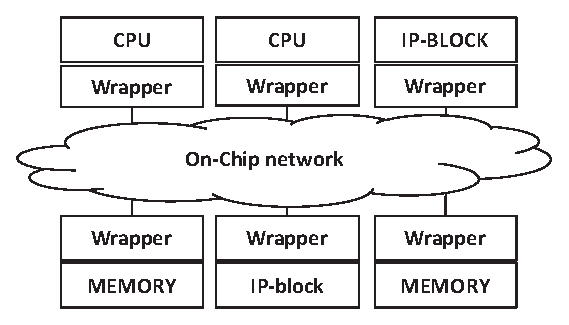
\includegraphics[width=0.60\textwidth]{../Fig/Eps/fig_soc_concept.eps}}
    \caption{Conceptual structure of system-on-chip}
    \label{fig:soc_concept}
  \end{center}
\end{figure}

\subsection{Main points}
The major design choices for HIBI were 
\begin{itemize}
\item	IP-block granularity for functional units
\item	Application independent interface to allow re-use of processors and IP-blocks
\item	Communication and computation separated
\item	Communication network used in all transfers, no ad-hoc wires between IPs
\item	support local clock domains for IP granularity
\end{itemize}

A parameterizable HW component, called HIBI wrapper, is used to
construct modular, hierarchical bus structures with distributed
arbitration and multiple clock domains as shown in Fig
\ref{fig:hierarchy} (explained later in detail).  This simplifies
design and allows reuse since the same wrapper can always be utilized.
Configuration takes place both at synthesis time (e.g. data width and
buffer sizes) and on runtime (arbitration parameters).

In addition, since we are targeting also FPGAs, there are some additional constraints
\begin{itemize}
\item	keep the number of wires low - to avoid exhausting routing resources
\item	avoid global connections - to avoid long combinatorial routing delays
\item	avoid 3-state wires - to simplify testing and synthesis (most FPGAs allow three-state logic onlu in I/O pins)
\end{itemize}


\subsection{Versions}
The development of HIBI \cite{kuusilinna98, lahtinen02, lahtinen04,
  salminen10} started in 1997 in Tampere University of Technology.
Currently, there are 3 versions of HIBI, denoted as v1-v.3. However,
certain basics have remained unchanged. Hence, in the remainder the
version number is omitted unless, it is necessary.

In version 2, the biggest changes were removing tri-state logic and
increasing modularity and configurability.

For version 3, address decoder logic was modified to simplify
usage. Furthermore, the tx and rx state machines were re-factored,
which also necessitated minor change in bus timing. These latter FSM
changes do not affect the IP, though.




\section {HIBI topology}

\begin{figure*}
  \begin{center}
    {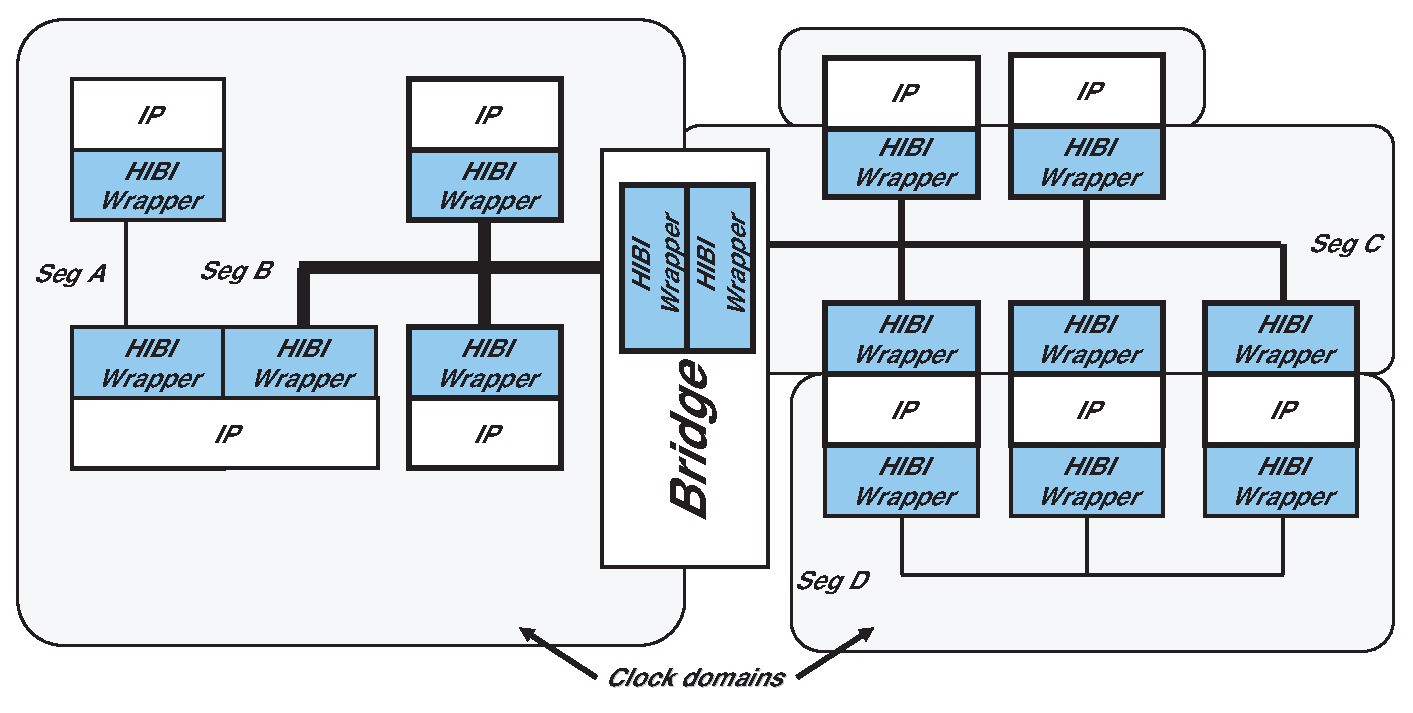
\includegraphics[width=0.85\textwidth]{../Fig/Eps/fig_topo_hibi_hierarchy.eps}}
    \caption{Example of a hierarchical HIBI network with multiple clock domains and bus segments}
    \label{fig:hierarchy}
  \end{center}
\end{figure*}


The topology in HIBI is not fixed, but configurable by the
designer. HIBI network consists of wrappers, bus segments, and
bridges. These are the basic building blocks from which the whole
network is constructed and configured.  All wrappers in the system are
instantiated from the same parameterizable HDL (HW description
language) entity and bridges are constructed by connecting two
wrappers together.  If the connected segments use different data
widths, the bridges are responsible for the data width adaptation.

All wrappers can act both as a \textit{master} and a
\textit{slave}. Masters can initiate transfers and slaves can only
respond. In many buses, most units operate in on mode only and only
few in both modes. In the most simple case, there is only segment and
the topology is hence single shared bus. However, HIBI network can
have multiple segments which form a hierarchical bus
structure. Segments are connected together using bridges. Bridges
increase latency but, on the other hand, hierarchical structure allows
multiple parallel transactions. Bridge are simply constructed from 2
wrappers.

For the IP, the wrapper offers FIFO-based (first in, first out)
interface, as depicted in Fig.  In network side, all signals inside a
segment are shared between wrappers and no dedicated point-to-point
signals are used. Arbitration decides which wrapper (or bridge)
controls the segment and the utilized arbitration algorithms
distributed to wrappers without any central controller. 

\subsection{Example of hierarchical topology}

Bus performance can be scaled up by using bridges. Segments having
only simple peripheral devices can have a slow and narrow bus while
the main processing parts have higher capacity buses.

Fig.~\ref{fig:hierarchy} depicts an irregular HIBI network. The
example has a point-to-point link ($Seg A$), hierarchical bus ($Seg B$
and $SegC$), and multibus topology ($Seg C$ and $SegD$). Furthermore,
$Seg B$ is wider than other segments and thus offers greater
bandwidth.  In the multibus configuration, each IP must decide which
bus to use while sending. Note that $Seg A$ could be implemented
without wrappers since there is no need for arbitration.

The example shows four clock domains. Agents in $Seg A$ and $SegB$ are
inside one domain and HIBI wrappers on $Seg C$ are in one domain.
However, two IPs in the top right corner use different clock than the
wrappers of $Seg C$.  The IPs in the bottom right corner and all
wrappers in $Seg D$ are in one domain.  The number of clock domains is
not otherwise restricted but all wrappers in one bus segment must use
the same clock. Handshaking between the clock domains is done in the
IP-wrapper interface or inside the bridge \cite{kulmala06b,
  kulmala06e}. This allows the construction of GALS systems. The
example shows only one bridge but HIBI does not restrict either the
number of bridges or hierarchy levels in contrast to many bus
architectures.

\subsection{Switching}
Transfers inside a bus segment are circuit-switched and use a common
clock due to (current) implementation of the distributed arbitration.
However, HIBI bridges utilize switching principle that resembles
packet-switching so that bus segments are not circuit-switched
together.  Instead, the data is stored inside the bridge until it gets
an access to the other segment. The data is forwarded to next segment
as soon as possible like in wormhole routing. However, no guarantees
are given for the minimum length of continuous transfer.  If the
bridge cannot buffer all the data, the transfer is interrupted and the
source segment is free for other transfers.  The interrupted wrapper
will continue the transfer on its next turn.  It is also possible that
a bridge buffers parts from multiple transfers.



\section {Data transfer operations}

In HIBI, all transfers are bursts. In practice, there is always 1
address word followed by n data words. The max. n is wrapper-specific
arbitration parameters. HIBI v2. used multiplexed address and data
lines, but HIBI v.3 allows transmitting them in parallel. Due to
multiplexed addr/data lines, it is beneficial to send many data into
single address. This is quite different from ``traditional'' memory
accesses, with address and data at the same time. Hence, the
destination IP should keep track of received data count, e.g. TUT's
SDRAM controller can do this to avoid excess transmitting addr + data
pairs

The transfers are pipelined with arbitration, and hence the next
transfer can start immediately when the previous ends. The protocol on
the bus side is optimized so that there no wait cycles are allowed
during a transfer. This means that is sender runs out of data or the
receiver does not accept it fast enough, the transfer is
interrupted. On the next arbitration turn, the wrapper it continues
automatically. Note that IP may transfer data at pace it wishes. IP
has only to ensure that there is space in TX FIFO while writing and
that RX FIFO is not empty while reading.

In order to increase bus utilization, HIBI uses so called
split-transactions in read operation. It means that single read
operation is split into two phases: request and response. The bus
segment is released while the addressed IP handles the read request
and prepares its response. The other wrappers may use bus during that
period and this increases the overall performance, although a single
read becomes a little slower due additional arbitration round.

\begin{figure}
  \begin{center}
    {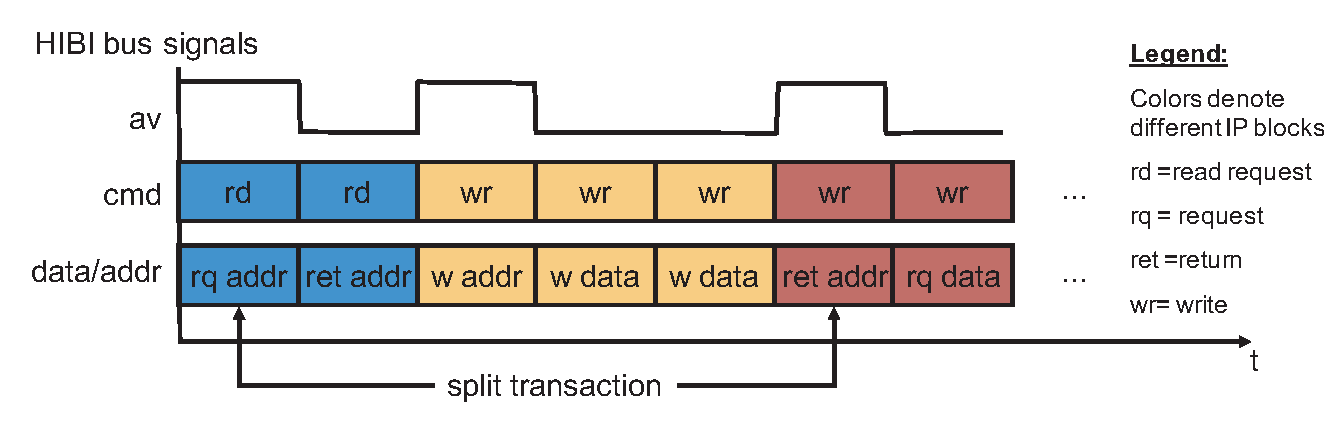
\includegraphics[width=0.7\textwidth]{../Fig/Eps/fig_basic_tx.eps}}
    \caption{Example of read and write operations.}
    \label{fig:basic_tx}
  \end{center}
\end{figure}

\begin{figure}
  \begin{center}
    {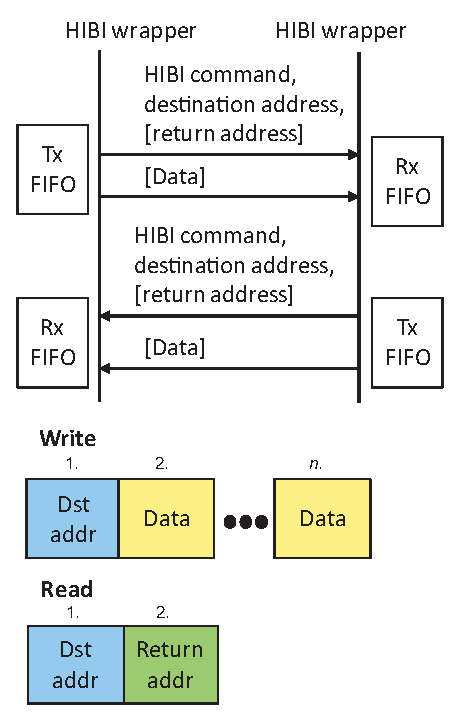
\includegraphics[width=0.4\textwidth]{../Fig/Eps/fig_basic_tx2.eps}}
    \caption{Basic transactions are write and read.}
    \label{fig:basic_tx2}
  \end{center}
\end{figure}


Write operation
\begin{itemize}
\item	Includes destination address
\item	Data is sent in words (=HIBI bus width)
\item	Several words can follow: all will be sent to the same destination address
\end{itemize}
Read operation
\begin{itemize}
\item	Includes exactly two words: destination address and return address (where to put the data)
\item	Data is received in words
\item	Several words can be received (all to same return address)
\begin{itemize}
\item	No handshaking: data is transmitted/received when bus, sender, or receiver are available
\item	No acknowledgements or flow control
\end{itemize}
\end{itemize}


Figs.~\ref{fig:basic_tx} and~\ref{fig:basic_tx2} depict the two basic
transfers: sending the read request, write, and the response to
read. IP can send multiple read requests before the previous ones have
completed. It is the responsibility of the requestor to keep track
which response belongs to which request. This can be implemented with
appropriate use of return addresses. The reader does not get data any
faster but the advantage is that the shared medium is available for
other agents in the middle of the transmission process and
consequently the achieved total throughput increases. In
packet-switched networks the split-transactions are commonly used and
also in modern bus protocols, such as AMBA

Since there is exactly one path between each source and destination,
all data is guaranteed to arrive in-order and hence no reordering
buffers are needed at the receiver.  Data can be sent with different
relative priorities. High priority data, such as control messages,
bypass the normal data transfers inside the wrappers and bridges
resulting in smaller latency. This does not change the timing of bus
reservations, but it selects what is transferred first.

\subsection{HIBI Basic Transaction Motivation}
HIBI was motivated by streaming applications where continuous flow of
data is transmitted between IPs. Destinations are merely ports than
random accessed memory locations. Hence, HIBI is not natively a
processor memory bus but can be used for it as well.

HIBI does not implement end-to-end flow control but the IPs must do
not explicitly. The FIFO buffers and rx and tx side may get full if
the receiver does not eject data fast enough, and this will throttle
the transmitter as well. The wrappers takes care of retransmission at
the link level. (HIBI v.1 dropped data if the receiving buffer got
full but usage of v.1 is not recommended anymore).


\begin{figure*}
  \begin{center}
    {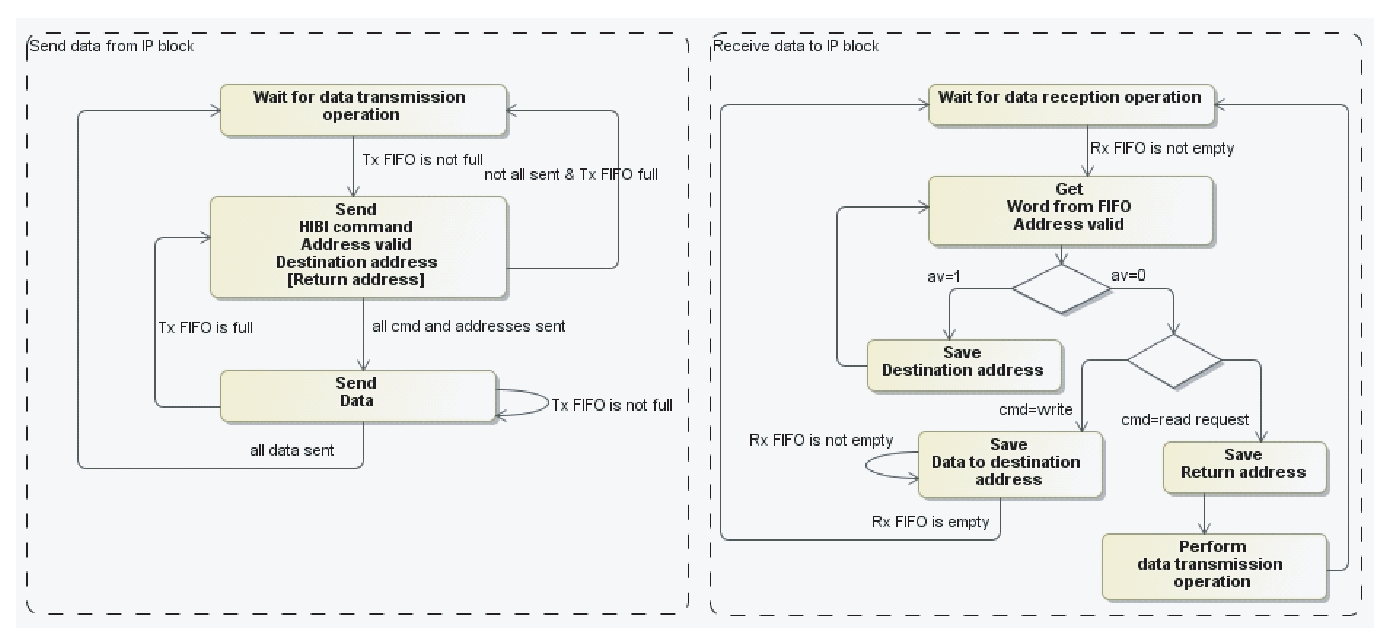
\includegraphics[width=0.8\textwidth]{../Fig/Eps/fig_tx_steps.eps}}
    \caption{Logical steps that IP does during transaction.}
    \label{fig:tx_steps}
  \end{center}
\end{figure*}

 
Fig.~\ref{fig:tx_steps} shows the steps that IP needs to take when
communicating using HIBI. On the left, IP sends data when the TX FIFO
is not full. It must assign data, address valid (strobe), command, and
write enable signals at the same time. When receiving data, IP first
checks is the incoming value address or data word. This is done by
examining the address valid signal. One word is removed from the FIFO
on every clock cycle when receiver assigns read enable signal. Next,
IP must check is the operation write or read. In case of write, it
stores the incoming data to location defined by the address. In case
of read, the second word denotes the return address. It is the
address, where the read data word must be transmitted.

\section{Addressing}

All IP-blocks have unique address and register space defined at design
time and every transfer starts with single destination address.
Source identification not included in basic transfer and hence

a)	Use data payload to define source, e.g. first world in a data packet

b) Use unique address inside IP block for each source (IP knows from
the destination address the sender)

Every wrappers has a set of addresses and they set with a VHDL generic
(automatic by Kactus).  Wrappers may have varying address space sizes,
e.g. simple UART has only 2 addresses whereas memory has 16K
addresses. Incoming Addresses go through the receiving wrapper to the
receiving IP and it can identify the incoming data by its address. For
example, the uppermost bits define which IP is addressed and the
lowermost define the register of that IP.

There are wo ways to set addresses 
1. manually

2. A generator script in Kactus tool does this automatically according
to system specification

IP may write arbitrarily long bursts to wrapper. Perhaps only one
address in the beginning followed by arbitrary number of data
words. Moreover, IP writes data in arbitrary pace to wrapper. There
can be any number of idle cycles between data words. Therefore, the
bursts sent by the IP do not necessarily have the same length in the
bus (between wrapper). For example, wrapper may split long IP-transfer
into multiple bus transfers if the arbitration algorithms gives
ownership to another wrapper in the middle. Each part of the transfer
starts with the same address as previous.  On the other hand, a
wrapper may send many short IP-transfers consecutively at one turn.

These properties have two consequences:

1. Bursts from multiple source IP will be interleaved

2. Destination may get different number of addresses than sender.

Note that the destination IP does not know the sender unless it is
separately encoded into data or address


\subsection{HIBI destination addresses and channels}

In HIBI v.2, all transfers are bursts, i.e. address is transmitted
only in the beginning of the transfer and it is followed by one or
more data words.  The maximum burst length is wrapper-specific. HIBI
uses mainly two-level addressing scheme: the upper bits of the address
identify the target terminal (e.g.  $destination_0$) whereas the lower
bits define the additional identifier. This identifier can be used
either as an address to local memory, to select the correct reception
channel on DMA, to identify the source of the data, or to select
requested service. Certain packet-switched networks (at least those
implemented in this work) allow only one address per terminal. In that
case, the second level address must increase the header length.


HIBI destination addresses are

1. internal registers

2. ports (to/from IPs internal logic)

3. IPs memory locations transparent to outside

Burst transfers use channels (or ports) and IP block must perform
addressing (increment) internally since all data is sent to one
address. If IP's memory is transparent, the address seen outside
includes also IP-block address (e.g. in address 0xB100, oxB000 defines
the target IP and 0x100 internal memory)


\begin{figure}
  \begin{center}
    {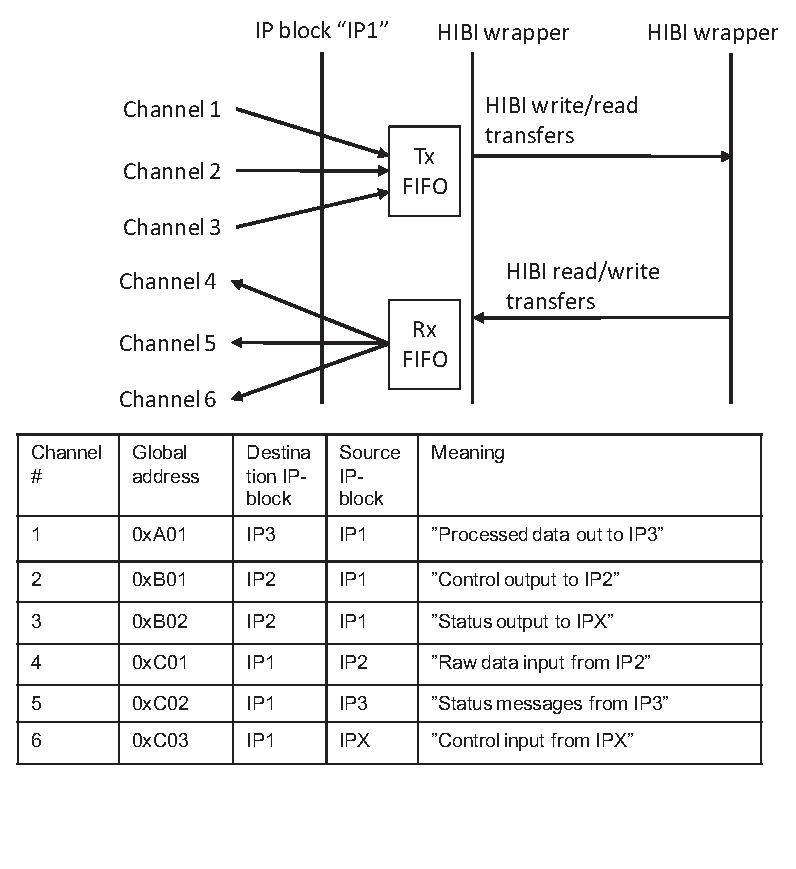
\includegraphics[width=0.5\textwidth]{../Fig/Eps/fig_chan_addr.eps}}
    \caption{Relation between addresses and channels.}
    \label{fig:chan_addr}
  \end{center}
\end{figure}



HIBI transfers can be abstracted as channels at IP-block side (but not
formally specified how). Easiest way to separate channels is to use
unique HIBI addresses. It is IP/System level design issue is to give
meaning to the channels. For example, accelerator receives data from
CPU0 via channel 0 and from CPU1 via channel 1 and so on. Basic HIBI
transactions are used to handle possible flow control and handshaking
in addition to transfers. Fig.~\ref{fig:chan_addr} shows an example
with 6 channels (addressing style of HIBI v.2) .

Note that all incoming channels 4-6 have the same 4 upper bits in
their addresses. In other words, the example uses a convention that
the base address of IP1 is 0xC00 and therefore its uppermost address
is implcitly 0xCFF. The channels can be easily distinguished from the
lowest address bits. In HIBI v.3 the addressing defined using two
parameters: start and end address. Designer can use the same addresses
as in HIBI v.2 based systems, but this scheme allows more freedom is
address definitions, which especially beneficial in hierarchical
systems

\subsection{Implementing flow control}

Flow control and handshaking must be implemented in IP-blocks. In practise leads to IP-block specific methods which must be carefully specified at design time.
Minimum issues to be agreed
\begin{enumerate}
\item	Sender identification (e.g. unique channel address ties Ip block and purpose together)
\item Transfer size
\item Size unit in addressing(bytes/words)
\item Are byte enables utilized
\item Messages for non-posted transactions (Acknowledgements to
  write/read)
\end{enumerate}

\subsection{Example: Overlapping and breaking transfers}

It was noted that the transfers may split due to arbitration.  Example
in Fig.~\ref{fig:addr_interleaving} clarifies the phenomenon. Let us
assume that IP 1 and IP 2 send data to IP 3. We notice that IP 1 gets
the first turn in the bus its two first data words arrive to IP
3. However, after that IP 3 gets two consecutive words from IP 2, then
from IP 1 and so on. Note that in realistic case, the arbitration
happens less frequently but the example highlights the issue.

\begin{figure}
  \begin{center}
    {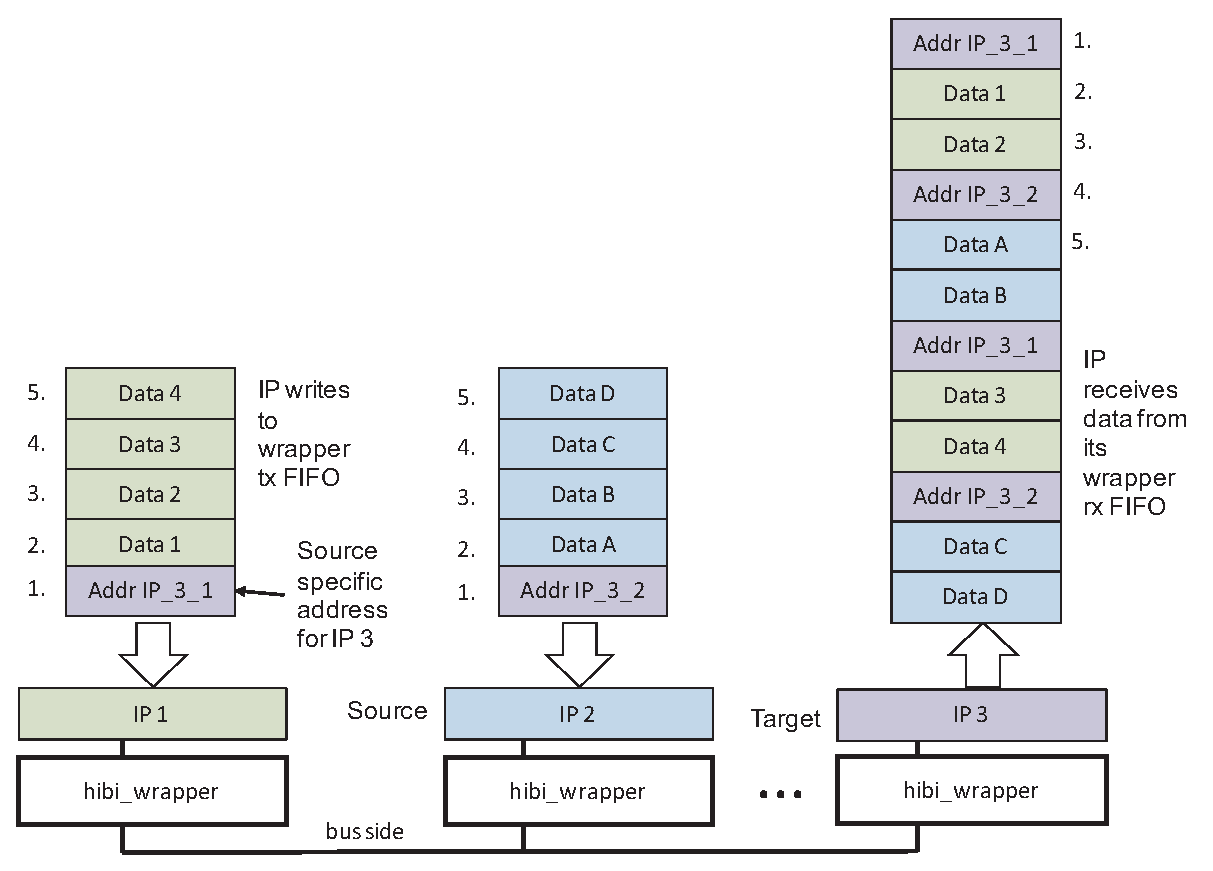
\includegraphics[width=0.5\textwidth]{../Fig/Eps/fig_addr_interleaving.eps}}
    \caption{The transfers may get intereleaved due to arbitration.}
    \label{fig:addr_interleaving}
  \end{center}
\end{figure}


\begin{figure*}
  \begin{center}
    {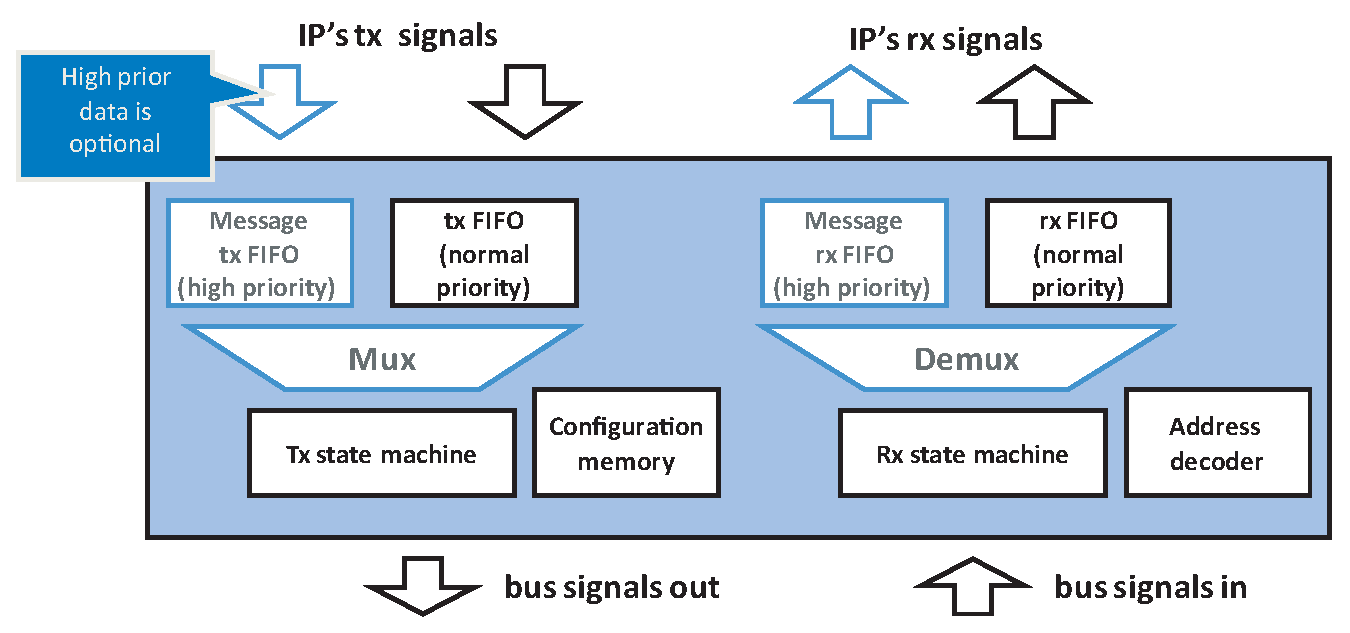
\includegraphics[width=0.65\textwidth]{../Fig/Eps/fig_hibi_wrapper.eps}}
    \caption{Structure of HIBI v.2 wrapper and configuration memory}
    \label{fig:wrapper}
  \end{center}
\end{figure*}


As a conclusion
\begin{enumerate}
\item Data is transferred in order through FIFO
\item If tx is interrupted in bus, wrapper re-sends address and
  continues tx of rest of data to destination
\item Sender tx FIFO can not be cleared once written
\item Receiver can identify to which channel data is coming based on
  address
 \end{enumerate}

\section{Wrapper structure}

HIBI network is constructed using parameterizable builgin blocks
called wrappers. The wrappers take care of arbitration, link-level
transmission, data buffering, and optional clock-domain crossing. All
signals on both sides of the wrapper are unidirectional. For example,
there are separate multibit signals data\_in and data\_out. Let us
first consider the bus side, i.e. the signals between wrappers.

The structure of the HIBI v.2 wrapper is depicted in Fig
\ref{fig:wrapper}.  The modular wrapper structure can be tuned to
better meet the application requirements by using different versions
of the internal units or leaving out properties that are not needed in
a particular application.

On IP side, there can be separate interfaces for every data priority
or they can be multiplexed into one interface.  Furthermore, the power
control signals can be routed out of the wrapper if the IP block can
utilize them.


The main parts are buffers for transferring and receiving data and the
corresponding controllers. The transfer controller takes care of
distributed arbitration. The configuration memory stores the
arbitration parameters. Relative data priority is implemented by
adding extra FIFOs. A (de)multiplexer is placed between the FIFOs and
the corresponding controller so that the controller operates only on a
single FIFO interface.  The separate (de)multiplexer allows adding
FIFOs to support priorities in excess of two without changing the
control. Currently, transmit multiplexer uses pre-emptive scheduling.



HIBI v.2 has multiplexed address and data lines whereas HIBI v.1 uses
separate address and data lines. Multiplexing decreases implementation
area because signal lines are removed and less buffering capacity is
needed for the addresses.  This causes overhead in control logic but
that is less than the saving in buffering.  Having fewer wires allows
wider spacing between wires and hence lower coupling capacitance.  On
the other hand, the saved wiring area can be used for wider data
transfers to increase the available bandwidth.  The HIBI protocol does
not require any specific control signals, but message-passing is
utilized when needed. HIBI v.1 assumes strictly non-blocking transfers
and omits handshake signals to minimize transfer latency but one
handshake signal \textit{Full} was added to HIBI v.2 to avoid FIFO
overflow at the receiver.  As a result, blocking models of computation
can be used in system design and, in addition, the depths of FIFOs can
be considerably smaller than in HIBI v.1.

\subsection{Bus-side signals}

All outputs from wrappers are ``ORed'' together and OR-gates' outputs
are connected to all wrappers' inputs. This scheme avoids the
tri-state logic that was used in HIBI v.1.
Table~\ref{table:bus_signals} lists the bus side signals and
Fig.~\ref{fig:3_wrappers} illustrates the connection between wrapper
and OR-gates. The cycle-accurate bus timing is omitted from this used
guide for brevity. All bus side outputs come directly from register
except the handshaking signal full.


\begin{table*}
  \caption {The signals at bus side, i.e. between the wrappers, in
  \label{table:bus_signals}
    v.2  and v.3 }
  \begin{center}
    \begin{tabular}{l | l | l | l}
      \hline
      Signal & Width   & Dir. & Meaning \\
      \hline \hline
      data   & generic & i+o  & Data and address are multiplexed into single set of wires \\
      av     & 1       & i+o  & Address valid. Notifies when address is transmitted \\
      cmd    & 3       & i+o  & Command: read or write, data or conficuration etc. \\
      full   & 1       & i+o  & Target wrapper is full and acannot accept the data. Current transfer will be repeated later \\
      lock   & 1       & i+o  & Bus is reserved \\
      \hline
    \end{tabular}
  \end{center}  
\end{table*}


\begin{figure*}
  \begin{center}
    {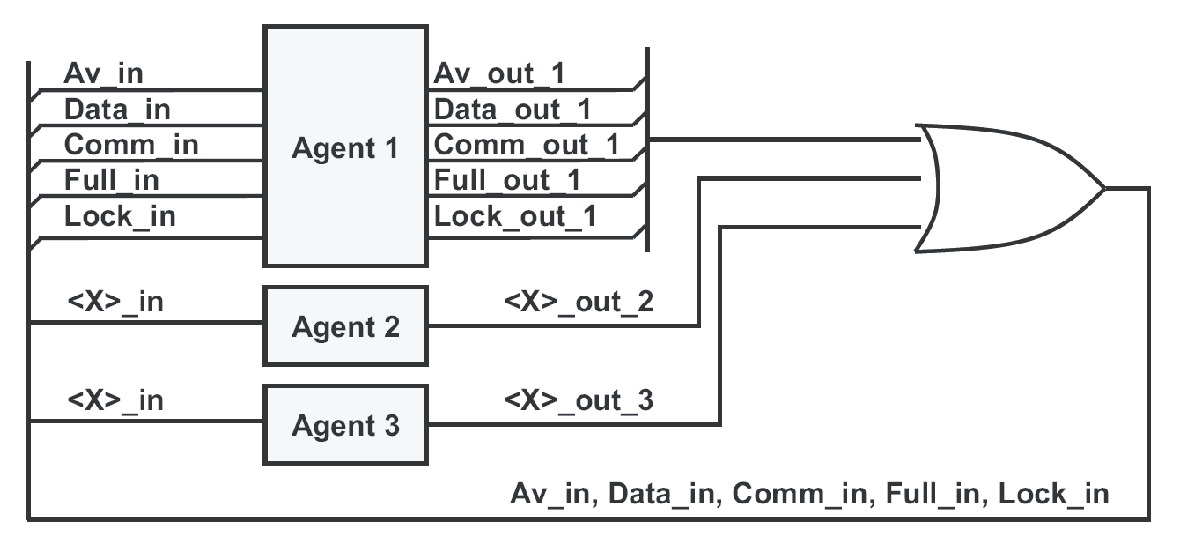
\includegraphics[width=0.65\textwidth]{../Fig/Eps/fig_hibi_3_wrappers.eps}}
    \caption{Structure of HIBI v.2 wrapper and configuration memory}
    \label{fig:3_wrappers}
  \end{center}
\end{figure*}

The number of data bits can be freely chosen.  This is beneficial, for
example, when error correcting or detecting codes are added to data
and the resulting total data width is not equal to any power of two.
Active master asserts $Lock$ signal when it reserves the bus.
Handshaking is done with the $Full$ signal. When $Full$ is asserted,
the data word on the bus must be retransmitted by the wrapper.  To
improve modularity, all signals are shared by all wrappers within a
segment and no point-to-point signaling is required. Consequently, the
interface of a wrapper does not depend on the number of agents and the
wrapper can be reused more easily.  An OR network was selected for bus
signal resolution.

The HIBI implementation pays special attention on minimizing the
transfer latency by removing empty cycles from the arbitration process
by pipelining.  Empty cycles are here defined as cycles when at least
one wrapper has data to send but the bus segment is not reserved.  An
optimized protocol allows lower frequency, and hence lower power, for
certain performance level than inefficient protocol.  Empty cycles
appear also when bus utilization is low as distributed round-robin
arbitration takes one cycle per agent. If only one agent is
transmitting, it has to wait a whole round-robin cycle between
transfers. In such cases, the priority-based arbitration is useful.


\subsection{IP-side signals}
The signals at IP interface are mostly the same signals as in the bus side. Interface signals are connected to FIFO buffers inside the wrapper  and all output signals of the wrapper come from registers. 

Most signals are driven by both IP and wrapper
\begin{itemize}
\item	Command
\item	Address / Address valid
\item	Data
\begin{itemize}
\item	May have high (message) and low (data) priotities (depends on wrapper type)
\item	Priority is defined by transmissting IP-block (source)
\end{itemize}
\end{itemize}

On the other hand, the FIFO access control signals depend on the
direction. Both control signals Write enable and Read enable and
driven by wrapper. The status signals are driven by wrapper. There are
always at least two status signals FIFO full and FIFO empty. In
addition, the FIFO buffers developed for HIBI offer two others: One
data left at FIFO and One place left at FIFO, which may simplify the
logic IP.

The address signals at IP side offer few choices that described next.

\begin{figure*}
  \begin{center}
    {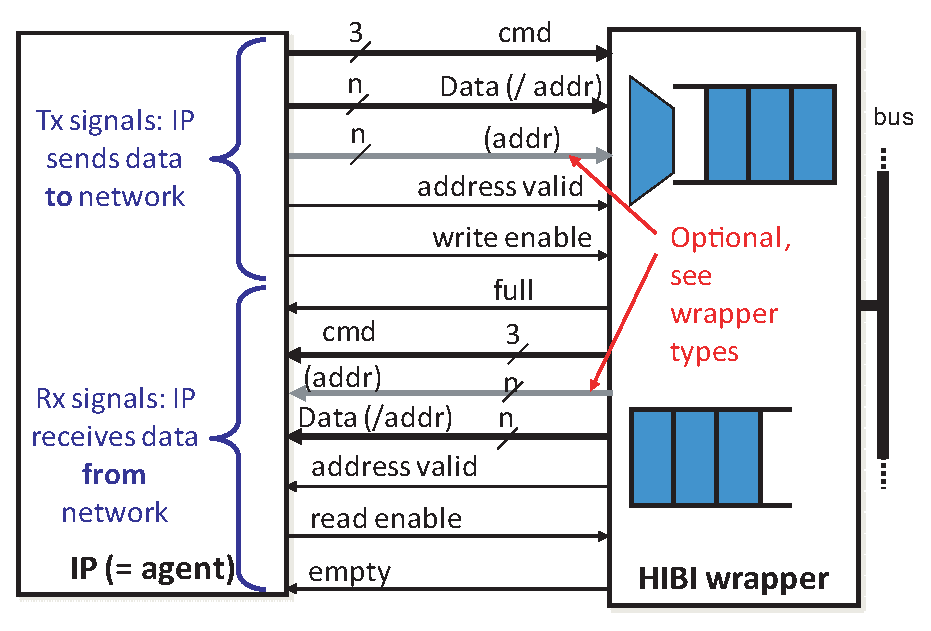
\includegraphics[width=0.6\textwidth]{../Fig/Eps/fig_ip_signals.eps}}
    \caption{The signals between IP and wrapper}
    \label{fig:ip_signals}
  \end{center}
\end{figure*}

Fig~\ref{fig:ip_signals} depicts the signals between IP and wrapper and
Table~\ref{table:ip_signals} list their details.

\begin{table*}
  \caption {The signals at wrapper's IP interface}
  \label{table:ip_signals}
  \begin{center}
    \begin{tabular}{l | l | l | l}
      \hline
      Signal & Width   & Dir. & Meaning \\
      \hline \hline
      rst\_n & 1       & i    & Active low reset \\
      clk    & 1       & i    & Clock, active on rising edge. Same for all wrappers inside one segment \\
      data   & generic & i+o  & Data and address are multiplexed into single set of wires \\
      av     & 1       & i+o  & Address valid. Notifies when address is transmitted \\
      cmd    & 3       & i+o  & Command: read or write, data or conficuration etc. \\
      re     & 1       & i    & Read enable. Wrapper can remove the first data from FIFO \\
      we     & 1       & i    & Write enable. Adds the data from IP to TX FIFO \\
      full   & 1       & o    & TX FIFO is full \\
      empty  & 1       & o    & RX FIFO is empty \\ 
      one\_p & 1       & o    & TX FIFO has one place left, i.e. almost full \\
      one\_d & 1       & o    & RX FIFO has one data left, i.e. almost empty \\
      \hline
    \end{tabular}
  \end{center}  
\end{table*}


\subsection{Variants of IP interface}
There are 4 variants of the IP interface depending on how to handle

a) high/low priority data: one or two interfaces

b) address and data: separate interfaces or one multiplexed

The different wrapper are denoted with postfix $\_r<x>$

r1: a) 2 interfaces  hi+lo; 	b) muxed     a/d

r2: a) 1 interface   hi/lo; 	b) separate  a+d

r3: a) 2 interfaces  hi+lo;  	b) separate  a+d

r4: a) 1 interface   hi/lo;    	b) muxed     a/d 

Since these options affect only the IP side, different wrapper types
can co-exist in the same system, and the wrappers' bus side interface
is always the same. Furthermore, the addresses work directly between
wrapper types. However, hi-priority data cannot bypass lo-prior data
in wrapper types r2 and r4. However, all data is always transmitted

For example, Nios subsystems utilize commonly r4 but SDRAM utilizes
r3. This is because SDRAM ctrl distinguishes DMA configuration and
memory data traffic with priority of incoming data. It also prevents
dead-lock. Fig ~\ref{fig:ip_interface_variants} depicts variants of
wrapper's IP side signals. Interface type r1 is the ``native''
interface that is used inside all other variants.

\begin{figure*}
  \begin{center}
    {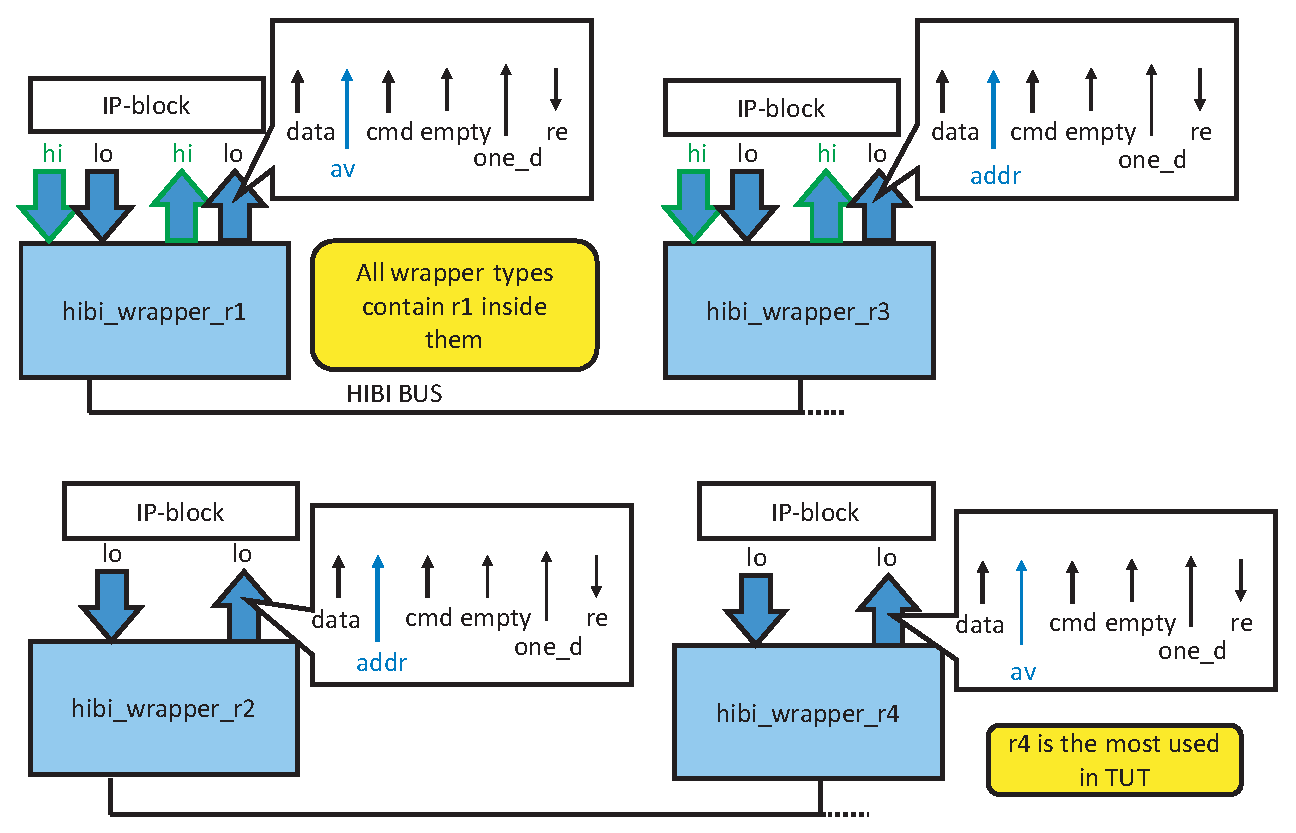
\includegraphics[width=0.8\textwidth]{../Fig/Eps/fig_ip_interface_variants.eps}}
    \caption{There are 4 variants of IP interface. There are two
      selectable features, namely separations of hi/lo-prior data and
      separate/multiplexed addressing.}
    \label{fig:ip_interface_variants}
  \end{center}
\end{figure*}

\subsection{Signal naming in VHDL}
The side and direction are marked into signal name in HIBI wrapper VHDL, for example
\begin{enumerate}
\item agent\_data\_in, agent\_data\_out,
\item bus\_data\_in, bus\_data\_out
\end{enumerate}
Fig.~\ref{fig:sgn_naming} clarifies the naming scheme.

\begin{figure*}
  \begin{center}
    {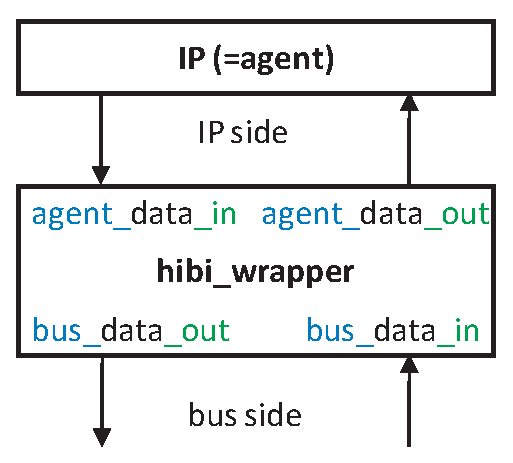
\includegraphics[width=0.5\textwidth]{../Fig/Eps/fig_sgn_naming.eps}}
    \caption{The naming convention of ports}
    \label{fig:sgn_naming}
  \end{center}
\end{figure*}

\subsection{Cycle-accurate timing}

For brevity, only the IP side timing is explained. It is actually very simple.
The timing when transmitting is depicted in Fig
1)	IP checks that tx FIFO is not full 
2)	IP sets data, command, addr/av, and write\_enable=1 for one clk cycle

\begin{figure*}
  \begin{center}
    \subfigure[IP sends.]{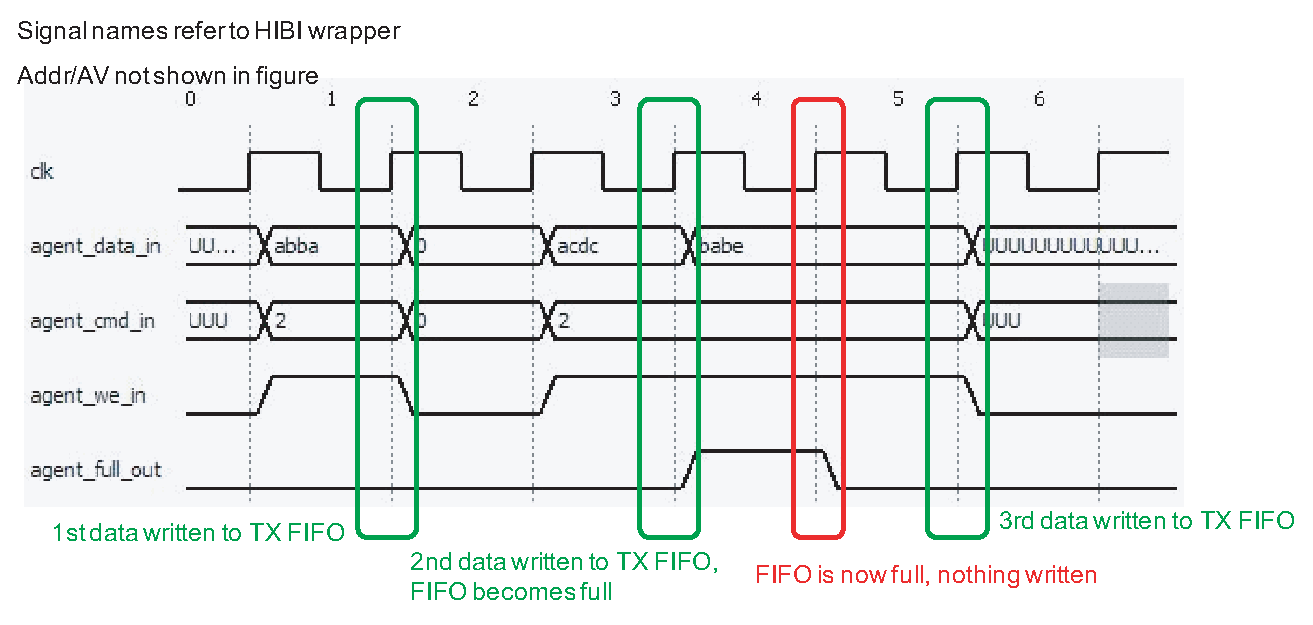
\includegraphics[width=0.95\textwidth]{../Fig/Eps/fig_tx_timing.eps}
      \label{subfig:tx_timing}}
    \subfigure[IP receives data]{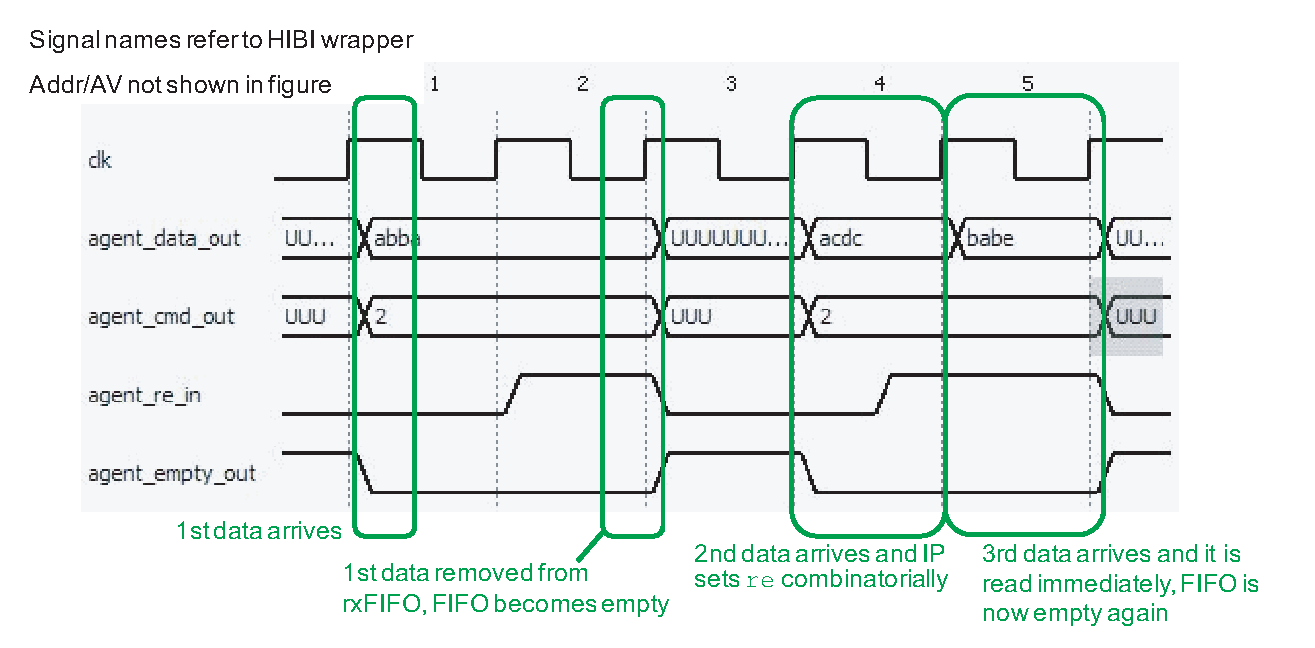
\includegraphics[width=0.95\textwidth]{../Fig/Eps/fig_rx_timing.eps}
      \label{subfig:rx_timing}}
    \caption{Examples of timing at IP interface.}
    \label{fig:interface_timing}
  \end{center}
\end{figure*}

The timing when receiving is depicted in Fig
1)	IP checks that rx FIFO is not empty
2)	IP captures data, command, and addr/av
3)	IP sets read\_enable=1 for one clk cycle



Notes on signal timing 
\begin{enumerate}
\item	Very easy to write/read on every other cycle
\item Almost as easy to write/read on every cycle. Needs a bit more
  care with checking empty and full
\item IP may keep we=1 and re=1 continuously and just change/store
  data according to full/empty
\item Signal FIFO full comes from register. It goes high on the next
  cycle after the write, if at all. In the Tx example, writing value
  0xacdc filled the FIFO
\item	Setting we=1 when FIFO is full has no effect
\item	Setting re=1 when FIFO is empty has no effect
\item Received data, addr/av and command appear to interface, if FIFO
  was empty before. IP can use them directly. They are ``removed'' only
  when read enable is activated o Checking empty==0 ensures validity
\item Data and command values are undefined when FIFO is empty. Most
  likely the old values remain
\end{enumerate}

A Simple example VHDL code can be found in SVN
/release\_1/lib/hw\_lib/ips/computation/image\_xor/tb/tb\_image\_xor\_linemaker.vhd
It shows how to send address and data. 

Fig.~\ref{fig:ip_fsm} shows the simple example FSM of the IP.
\begin{figure*}
  \begin{center}
    {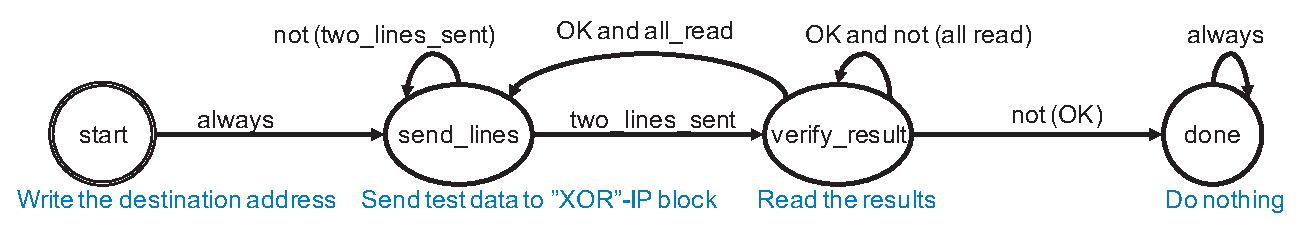
\includegraphics[width=0.9\textwidth]{../Fig/Eps/fig_ip_fsm.eps}}
    \caption{Example FSM of an IP}
    \label{fig:ip_fsm}
  \end{center}
\end{figure*}

Sometimes the output registers of the IP may cause unexpected behavior
for novices. Even if FIFO appears ``not full'', IP cannot necessarily
write new data. That happens if it was already writing and there was
only one place left at the FIFO. Hence, remember to check if IP is
already writing!

The following code snippet should clarify correct writing
\begin{lstlisting}[language=vhdl, style=console, basicstyle=\footnotesize, 
    title={Example code of IP's sending control}]
if (we_r ='1' and one_p_in='1') or full_in ='0' then
 we_r   <= '0'; //FIFO is becoming or already full
else 
 we_r   <= '1'; // There is room in FIFO
 data_r <= new_value; 
end if;
\end{lstlisting}




HIBI wrapper shows the data as soon as it comes from the bus. Same
data might get used (counted) twice, if IP only checks the empty
signal. Remember to check if IP is already reading!  The following
code snippet should clarify correct reading

\begin{lstlisting}[language=vhdl, style=console, basicstyle=\footnotesize, 
    title={Example code of IP's reception handling}]
if (re_r = '1' and one_d_in = '1') or empty_in = '1' then
 re_r <= '0'; // Stop reading
else
 re_r <= '1'; // Start or continue reading
end if;

if re_r = '1' then
 if hibi_av_in = '0' then
  // handle the incoming address
 else
  // handle the incoming data
 end if;
end if;
\end{lstlisting}

Common pitfalls
\begin{itemize}
\item Not noticing that tx FIFO fills while writing. Consequence: Some
  data are lost (not written to FIFO)
\item Write enable remains 1 for one cycle too long. Undefined data
  written to FIFO, or the same data is written twice o In both of
  above, the likely cause is not acocunting to output register of the
  IP
\item Not noticing that rx FIFO goes empty while reading. Data
  consumed by IP is undefined
\item Read enable remains 1 for one cycle too long. Next data is
  accidentally read away from the FIFO unless FIFO was empty
\item Not noticing that rx data changes only after the clock edge when
  re=1. IP uses the same data twice
\end{itemize}





\section{Arbitration}
A distinct feature in HIBI is that arbitration is distributed to
wrappers, meaning that they can decide the correct time to access the
bus by themselves. Therefore, no central arbiter is required.  In
practice, Bus is ``offered'' to one wrapper on each cycle. The wrapper
reserves the bus using signal lock if has data to send.

Multiple policies are supported
\begin{enumerate}
\item	Fixed priority, Round-robin
\item	Dynamically adaptive arbitration (DAA)
\item	Time-division multiple access (TDMA)
\item	Random 
\item	Combination of above
\end{enumerate}

A scheme called Dynamically Adaptive Arbitration (DAA) was presented
in \cite{kulmala08b}. In most cases, designers should use round-robin
or DAA. If there is minor performance bottleneck, one can easily
configure the arbitration parameters.

\begin{figure*}
  \begin{center}
    {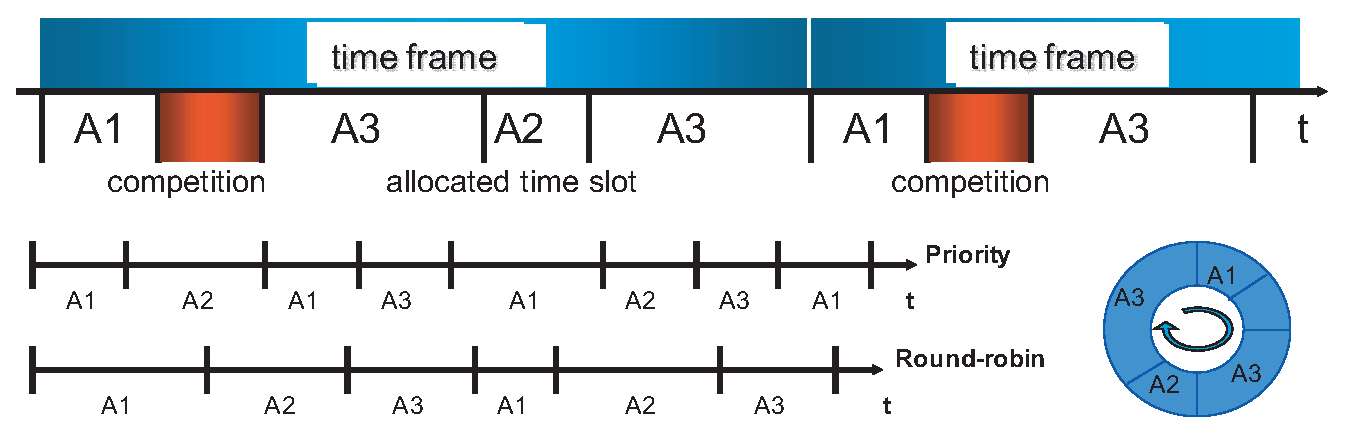
\includegraphics[width=0.8\textwidth]{../Fig/Eps/fig_arb_example.eps}}
    \caption{Example timing in 3 arvitration policies.}
    \label{fig:arb_example}
  \end{center}
\end{figure*}


Fig.~\ref{fig:arb_example} shows an example of different policies.  A
two-level arbitration scheme, a combination of time division multiple
access (TDMA) and competition, is used in HIBI.  In TDMA, time is
divided into repeating time frames. Inside frames, agents are provided
time slots when they are guaranteed an access to the communication
channel.  This way the throughput of each wrapper can be guaranteed.
The worst-case response time for a bus access through TDMA is the
interval of the adjacent time slots. TDMA in HIBI supports two flavors
for handling the slots when there is no data send: keeping them or
releasing the bus for competition.
\begin{figure*}
  \begin{center}
    \subfigure[Low contention (send probability  ~4\% per agent).]{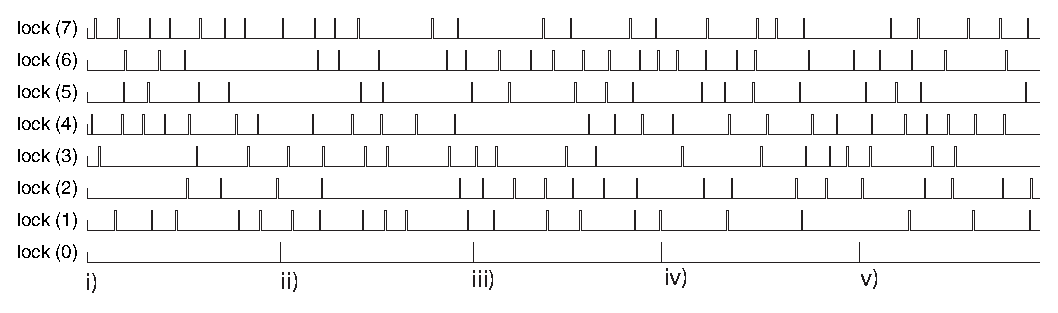
\includegraphics[width=0.85\textwidth]{../Fig/Eps/fig_arb_recfg_lowcontention_v2.eps}
      \label{subfig:wave_arb_lowcont}}
    \subfigure[High contention  (send probability ~30\% per agent).]{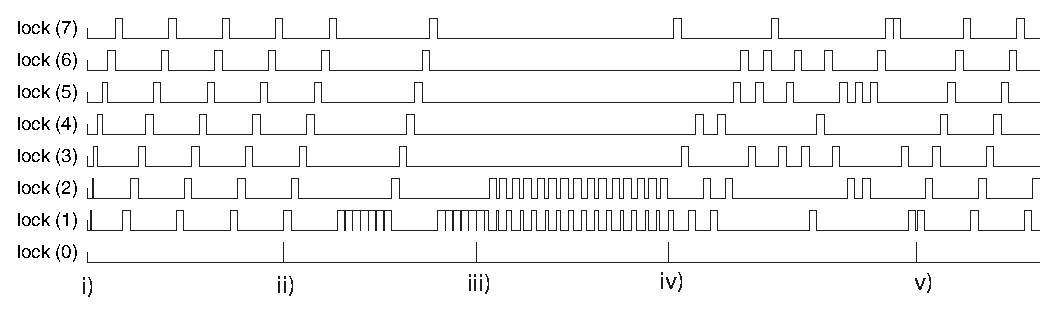
\includegraphics[width=0.85\textwidth]{../Fig/Eps/fig_arb_recfg_highcontention_v2.eps}
      \label{subfig:wave_arb_highcont}}
    \caption{Various arbitration schemes for 8-agent single bus and
      uniform random traffic. The differences become evident on highly
      utilized bus.}
    \label{fig:wave_arb}
  \end{center}
\end{figure*}


Competition is based either on round-robin or non-pre-emptive priority
arbitration. The second level mechanism is used to arbitrate the
unassigned or unused time slots.  If the agent does not have anything
to send in the beginning of its time slot, the time slot can be given
away to allow maximal bus utilization. Priority arbitration as a
second level method attempts to guarantee a small latency for high
priority agents whereas round-robin provides a fair arbitration
scheme.  When the bus is freed and priority scheme is utilized, the
agent with the highest priority can reserve the bus on the first
cycle. If the bus has been idle for two cycles, the agent with the
second highest priority may reserve it and so on.  The maximum
transfer length is restricted with runtime configurable parameter
$max\_send$.  For round-robin, the maximum wait time for accessing the
bus is obtained by summing all $max\_send$ values. For priority-based
arbitration, the maximum wait time can be defined only for the two
highest priorities.  This means that the low-priority agents may
suffer starvation and system may end up in deadlock.  Therefore, using
only priority arbitration is not recommended. 


\subsection{Detailed timing example}

Fig.~\ref{fig:wave_arb} shows the differences in various arbitration
policies and two traffic loads (low and high contention).  HIBI is
configured as single bus with 8 agents. Agent 0 performs dynamic
reconfiguration (time instants $i-v$) and other agents generate
uniformly distributed random traffic. The reconfiguration changes the
arbitration policy at runtime. The exact configuration procedure is
explained in more detail later %in Section\ref{ch:hibi:reconf}.
  The utilized arbitration policies are
\begin{enumerate}[i)]
\item round-robin
\item combination of priority and round-robin
\item priority
\item random
\item round-robin (again).
\end{enumerate}
Round-robin offers fair arbitration (each agent has its share) whereas
priority favors the highest priority agents and leads to starvation of
others. Their combination switches between them at user-defined
intervals. Arbitration policy does not play a major role when bus is
lightly loaded, as illustrated in Fig.~\ref{subfig:wave_arb_lowcont}.
The differences are clear with higher load,
Fig.~\ref{subfig:wave_arb_highcont}.

\subsection{Performance implications}

\begin{figure*}
  \begin{center}
    {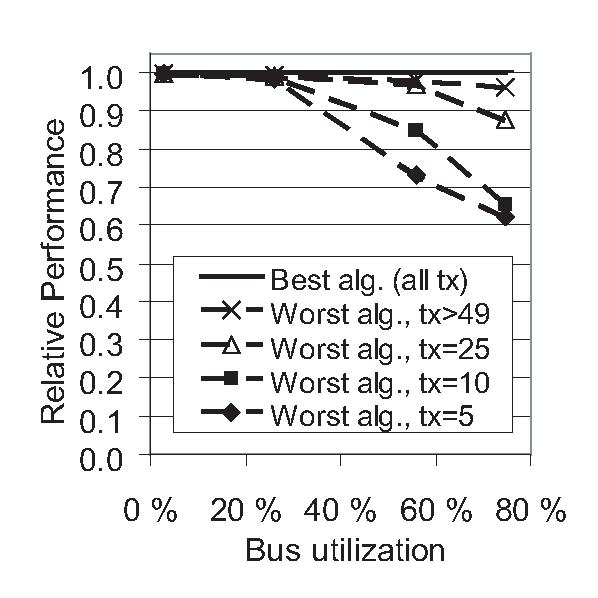
\includegraphics[width=0.5\textwidth]{../Fig/Eps/gra_hibi_arb_rel_perf.eps}}
    \caption{Relative performance of arbitration algorithms in MPEG-4
      encoding \cite{kulmala08b}}
    \label{fig:hibi_arb_rel_perf}
  \end{center}
\end{figure*}

% !!! ks. my�s $http://ieeexplore.ieee.org/iel5/10626/33561/01594751.pdf$

Various arbitration methods of HIBI were compared in
\cite{kulmala08b}.  The test case was MPEG-4 encoding on MPSoC. HIBI
has $6$ arbitrated components: $4$ CPUs, SDRAM, and performance
monitor; all operating at $50 MHz$ frequency.  The maximum transfer
length was varied from 5 words (denoted as $tx=5$) to non-limited.
Transfer length has major impact but all lengths of 50 words or over
(tx>49) resulted in equal performance.  The bus frequency was set to
$1, 2, 5$, or $50~MHz$ in order to achieve varying bus utilization
($75\%, 56\%, 26\%$, and $3\%$, respectively) with single application.
The best and worse algorithms vary case by case but DAA performed well
in general.

Fig.~\ref{fig:hibi_arb_rel_perf} plots the relative encoding
performance between the worst and best algorithms.  The curves denote
different transfer lengths, and $1.0$ is the best algorithm for each
case. Tx lengths over $49$ are joined for clarity because they yield
practically the same results. With short transfers, the worst
algorithm at $1~MHz$ HIBI ($75\%$ utilization) offers only $0.62x$ the
performance of the best, at $2~MHz~0.73x$, at $5~MHz~0.98x$, and at
$50~MHz$ there are no differences.

\section{Commands}


Source IP sets the command and most commands are forwarded to the receiving IP.
The most common commands are:
\begin{itemize}
\item	Write data - regular send operation, so called posted write
\item Read request - split-transaction, the requested data is returned
  later with regular write command
\end{itemize}
The other, less common commands are
\begin{itemize}
\item Idle - IPs never use this command, but this appears on the bus
  when no-one sends anything
\item High priority - bypasses normal data in the wrappers, otherwise
  just like regular operation, can be added to many commands
\item Write and read config - access the configuration memories inside
  the wrappers. Not forwarded to the IP at the receiving end
\item Multicast - send the same data to multiple targets (only in HIBI
  v.2)
\item Non-posted write - Receveir IP must provide some response (ACK
  or NACK) (v.3 only)
\item Linked read + conditional write - to perform
  read-modify-write (v.3 only)
\item Exclusive access - reserve the whole path to the destination,
  read, write, and remove the lock (v.3 only)
\end{itemize}

HIBI v.3 has 5 command bits and v.2 had only 3 bits,see
Tables~\ref{table:hibi_v3_cmd} and~\ref{table:hibi_v2_cmd}.

\begin{table*}
  \caption {The command codes in HIBI v.3}
  \label{table:hibi_v3_cmd}
  \begin{center}
    \begin{tabular}{l | l | r |l}
      \hline
      Cmd & Code  & Code     & Meaning \\
          & [4:0] & [decimal]&  \\
      \hline \hline
      idle             & 0 0000   & 0 & Appears on the bus when it is free    \\
      <reserved>       & 0 0001   & 1 & not used, most unused codes hidden from the table \\
      wr data          & 0 0010   & 2 & Regular write \\
      wr data hi-prior & 0 0011   & 3 & - `` - w/ high priority \\
      \hline
      rd data          & 0 0100   & 4 & Request of the split-transaction \\
      rd data hi-prior & 0 0101   & 5 & - `` - w/ high priority \\
      rd data linked   & 0 0110   & 6 &  \\
      rd d. linked hi-p& 0 0111   & 7 & - `` - w/ high priority \\
      \hline

      wr data non-post   & 0 1000   & 8  & Write that expects response\\
      wr d. non-post hi-p& 0 1001   & 9  & - `` - w/ high priority \\
      wr conditional     & 0 1010   & 10 & Write that follows rd linked \\
      wr cond. hi-p      & 0 1011   & 11 & - `` - w/ high priority \\
      \hline

%      <reserved>         & 0 1100   & 12 & not used \\
      excl. lock         & 0 1101   & 13 & Locks the path to the destination \\
%      <reserved>         & 0 1110   & 14 & not used \\
      excl. wr           & 0 1111   & 15 & Exclusive write, must follow excl.lock \\
      \hline
%      <reserved>         & 1 0000   & 16 & not used \\
      excl. rd           & 1 0001   & 17 & Exclusive read request, must follow excl.lock \\
%      <reserved>         & 1 0010   & 18 & not used \\
      excl. release      & 1 0011   & 19 & Removed the lock from the path\\
      \hline
%      <reserved>         & 1 0100   & 20 & not used \\
      wr config          & 1 0101   & 21 &  \\
%      <reserved>         & 1 0110   & 22 & not used \\
      rd config          & 1 0111   & 23 &  \\
      \hline
      <reserved>         & 1 1xxx   & 24-31 & not used \\
      \hline


      \hline
    \end{tabular}
  \end{center}  
\end{table*}


\begin{table*}
  \caption {The command codes in HIBI v.2}
  \label{table:hibi_v2_cmd}
  \begin{center}
    \begin{tabular}{l | l | l}
      \hline
      Cmd & Code [2:0] & Meaning \\
      \hline \hline
      idle             & 000   & Appears on the bus when it is free    \\
      wr config data   & 001   & Updates config mem inside the wrapper \\
      wr data          & 010   & Regular write \\
      wr data hi-prior & 011   & High-priority data bypasses the regualr one \\
      \hline
      rd data          & 100   & Request of the split-transaction \\
      rd config data   & 101   & Requests a value from wrapper's config mem \\
      multicast data   & 110   & Sends to all wrappers whose uppemost addr bits match \\ 
      multicast config & 111   & Same as above for high-priority data\\ 
      \hline
    \end{tabular}
  \end{center}  
\end{table*}


\section {Buffering and signaling}
The model of computation used in HIBI design approach assumes bounded
first-in-first-out (FIFO) buffers between processes. A simple FIFO
interface can be adapted to other interfaces such as the OCP
(Open Core Protocol)\cite{ocp03}. 
% The basic principle of OCP is shown in
% Fig \ref{fig:hibi_ocp}. 
% Transfers are initiated by $masters$ and $slaves$
% only respond to requests. The OCP transfers are translated to underlying
% network protocol, in this case HIBI, and back by OCP wrappers. 
% \begin{figure} [t]
% \begin{center}
% \includegraphics[width=0.7\textwidth]{../Fig/Eps/fig_hibi_ocp.eps}
% \caption{Using OCP with HIBI. The OCP interface is located between IP and HIBI wrapper}
% \label{fig:hibi_ocp}
% \end{center}
% \end{figure}
Consequently, IP components use only OCP protocol and are isolated
from the actual network implementation.  Ideally, network can be
chosen freely without affecting the IPs.  However, not all features of
HIBI, such as relative data priorities or dynamic reconfiguration, can
be used with OCP directly but only the basic transfers.

To avoid excess buffering or retransfers, the received data must be
read from the FIFO as soon as possible, for example by using a direct
memory access controller. As a result, the receiver buffer space is
not dictated by the \emph{amount} of transferred data, but the
\emph{latency} of reading data from the wrapper. This scheme resembles
wormhole routing, but the links are not reserved if the receiver is
stalled.

\section {Configuration}

HIBI is both modular and configurable. At design time: structural and
functional settings are made, whereas at run-time, one can modify data
transfer properties (arbitration types, wrapper specific QoS
settings).  

Fig.~\ref{fig:cfg_mem} shows the structure of the configuration
memory.
\begin{figure}
  \begin{center}
    {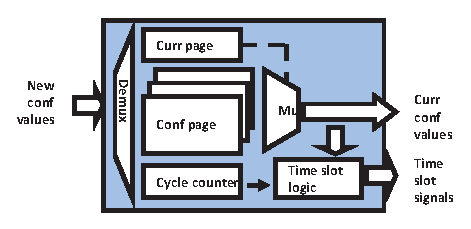
\includegraphics[width=0.5\textwidth]{../Fig/Eps/fig_cfg_mem.eps}}
    \caption{Structure of the wrapper's configuration memory}
    \label{fig:cfg_mem}
  \end{center}
\end{figure}

\subsection{Generic parameters in VHDL}
HIBI has a large set of generic parameters. They are categorized as
follows
\begin{enumerate}
\item Stuctural
  \begin{itemize}
  \item Widths of interface ports: data, command, debug port
  \item Widths of internal signals: address, wrapper identifier field,
    counters
  \item Sizes of tx and rx FIFOs, both lo and hi priorities
  \item	Use 0, 2, 3 etc.
  \item Run-time configuration: number of cfg pages, num of
    app-specific extra registers
\end{itemize}
\item Synchronization
  \begin{itemize}
  \item	Type of the synchronizing FIFO buffers
  \item Relative frequencies of IP and bus
\end{itemize}
\item	Functional
  \begin{itemize}
  \item Identifier, own address
  \item	For bridges: base identifier, inverted address space
  \item Arbitration: type, priority, how many words to at one turn,
    number of agents in the same segment
  \item For TDMA: number of time slots, how to handle unused slots
    (keep/give away)
  \item	Enable/disable multicast functionality
  \item Enable/disable runtime configuration functionality (affects
    structure=area as well)
  \end{itemize}
\end{enumerate}

Table~\ref{tab:generics} lists all the generics. Certain parameters
are system-wide settings, for example the width of the command. Some
are segment-wide, for example bus clock, data width, and number of
wrappers in that segment. The rest are instance-specific, for example
buffer sizes and priorities.
\begin{table*}
  \caption{Properties of HIBI v.1 and v.2.}
  \label{tab:generics}
  \begin{center}
    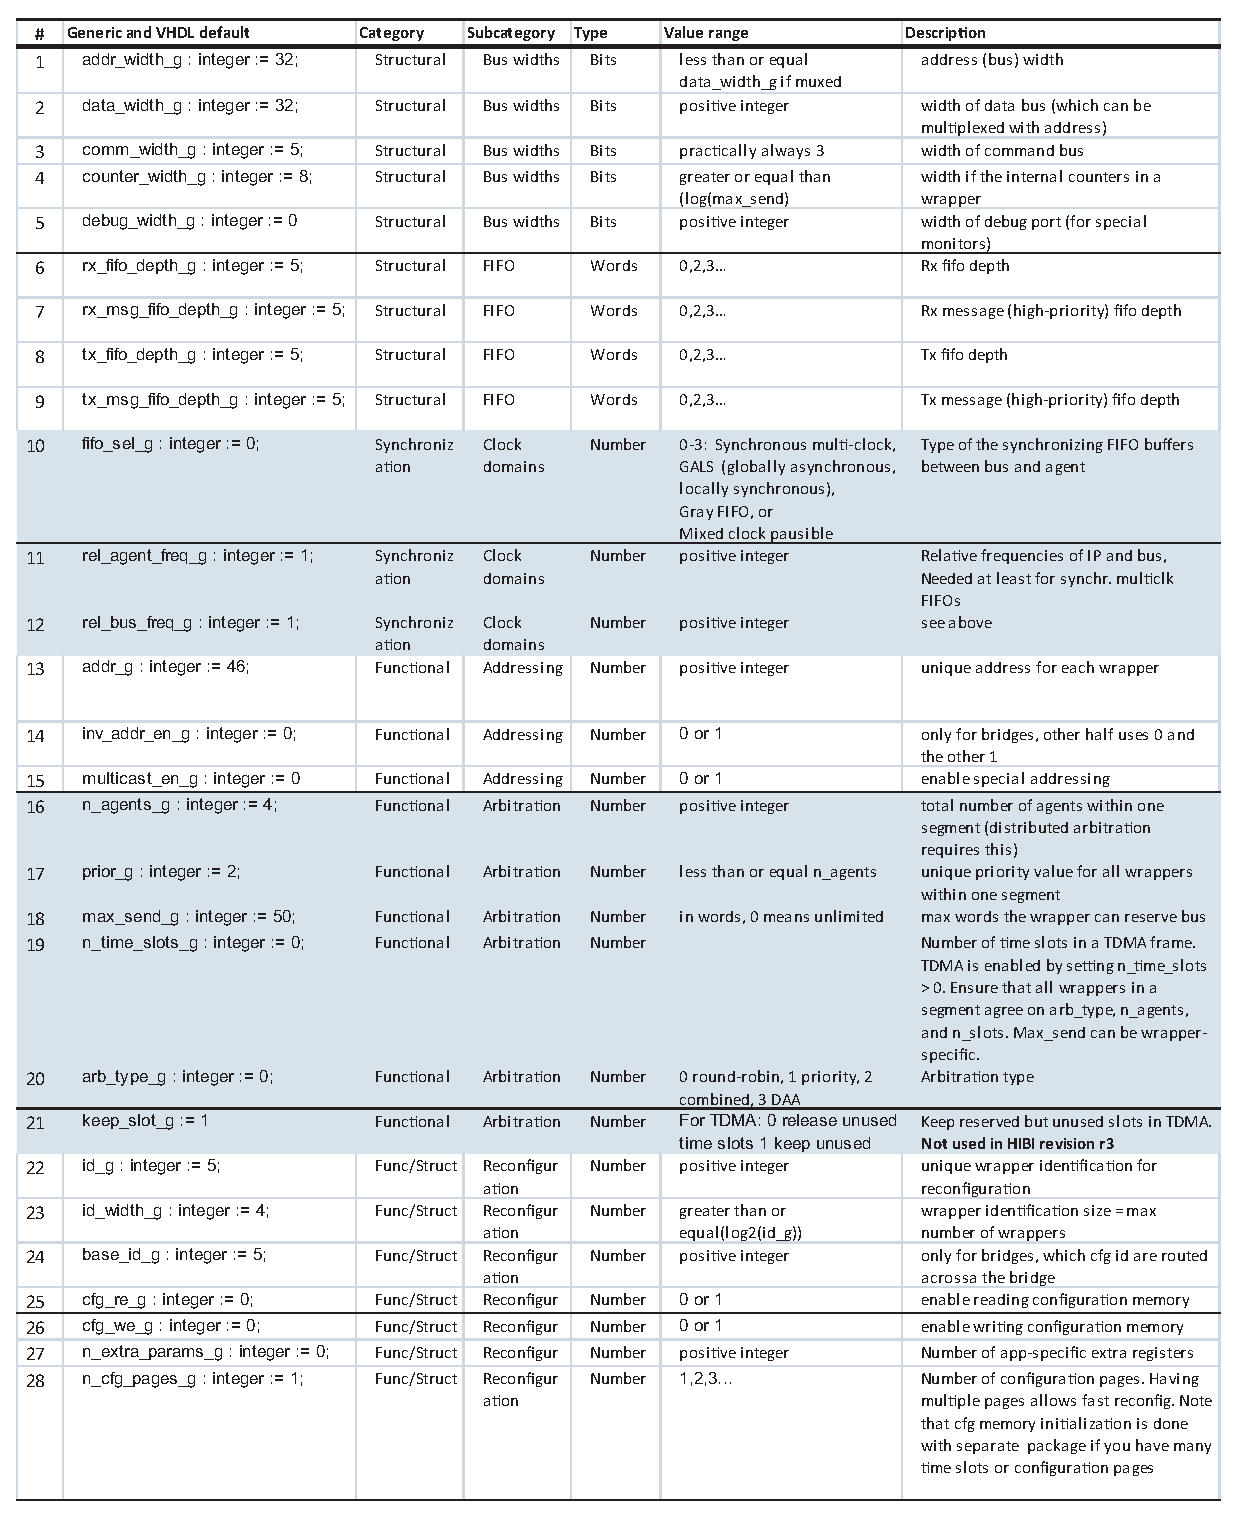
\includegraphics[width=0.95\textwidth]{../Fig/Eps/tab_generics.eps}
  \end{center}
\end{table*}


\subsection{Clocking}
HIBI can support may clock domains. The border is either between IP
and wrapper, or in the middle of a bridge. There are five options:
\begin{enumerate}
\item	Fully synchronous
\item Synchronous multi-clk: Clock frequencies are integer-multiples
  of each other. Clocks are in the same phase. Easy to use with FPGA's
  PLLs
\item GALS: No assumptions about relations (phase, speed) between
  clocks. Has longer synch. latency than synch.multiclock.
\item Gray FIFO: FIFO depth limited to power of two ($=2^n$)
\item Mixed clock pausible
\end{enumerate}

The method must be decide at synthesis time.

\subsection {Runtime reconfiguration}
\label{ch:hibi:reconf}
Wrapper has config memory that stores all information for
distributed arbitration. It can be synthesized in many ways:
\begin{itemize}
\item Permanent: ROM, 1 page
\item Partial run-time configurable: ROM with several pages
\item Full run-time configurable: RAM, with pages
\item Kactus supports currently 1-page ROM
\end{itemize}



HIBI allows the runtime configuration of all arbitration parameters to
maximize performance. This is achieved so that one of the agents (e.g.
system controller CPU) writes the new configuration values to all
wrappers. The configuration values are sent through the regular data
lines.  During the normal operation, i.e. when the configuration is
not changed, the controller CPU can perform its computation tasks.  In
the best case, other PEs can continue their transfers even if HIBI is
being configured. However, some operations, such as swapping
priorities of two wrappers, necessitate disabling other transfers
momentarily.


The structure of the configuration memory is illustrated at the bottom
of Fig \ref{fig:wrapper}.  It includes multiple configuration pages
for storing the parameter values, a register storing the number of
currently active page, clock cycle counter, and logic that checks the
start and end of times of the time slots.  The receive controller
takes care of writing new configuration values whereas the
configuration values and time slot signals are fed to the transfer
controller. Configuration values can be written to non-active pages
before they are used to minimize the risk of conflict when the
configuration is performed.




For very regular traffic, the TDMA slots can be set to minimize the
latency, i.e. slot starts shortly after the availability of data. For
TDMA, each wrapper has an internal cycle counter to decide correct
times to access the bus.  For this reason, wrappers in one bus segment
must be synchronized.  When data is produced with varying time
intervals or quantities, the time slots cannot be optimally located.
By runtime reconfiguration, the cycle counters can be reset to an
arbitrary clock cycle value within the time frame to keep time slots
in the correct place with respect to data availability. Also the
length and owner of the slots can be changed.  The resynchronization
can be triggered explicitly from software or automatically by a
specific monitor unit, which monitors how effectively time slots are
used and starts the reconfiguration if needed \cite{kangas02}.
Roughly 10 \% improvement in HIBI v.1 throughput in video encoding due
to dynamic reconfiguration was reported in \cite{lahtinen02}. Larger
gains are expected when several applications are executed on a single
platform.  Reconfiguration was used in \cite{kulmala08b} to speed-up
the exploration on FPGA. It allowed notably less synthesis runs, each
of which took several hours.

As a new feature in HIBI v.2, the second-level arbitration method can
be changed at runtime between priority and round-robin or both of them
can be disabled. When the second-level arbitration is disabled, only
the basic TDMA is used and the slot owner reserves the bus always for
the whole allocated time slot. Similarly, only the second-level
arbitration is utilized when no time slots are allocated.

\begin{figure*} [t]
  \begin{center}
    {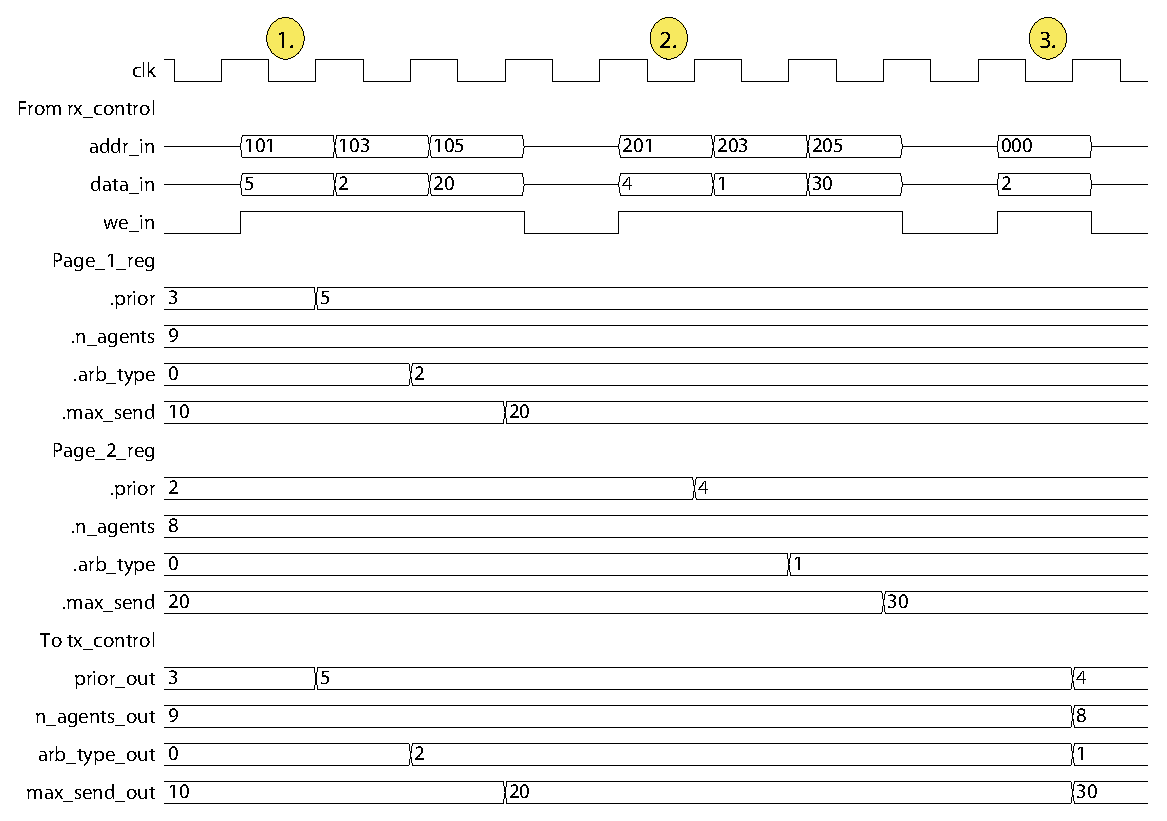
\includegraphics[width=0.75\textwidth]{../Fig/Eps/fig_hibi_cfg_mem_wave.eps}}
    \caption{Example of runtime configuration}
    \label{fig:cfg_mem_wave}
  \end{center}
\end{figure*}

In HIBI v.2, three methods are used to improve the configuration
procedure.  First, by making use of the bus nature, each common
parameter can be broadcast to all wrappers.  Second, enabling the
reading of configuration values simplifies the procedure as the whole
configuration does not have to be stored in the configuring agent.  In
contrast, the configuring agent can read the old parameter values to
help determining the new ones. Third, additional storage capacity for
multiple parameter pages has been added to enable rapid change of all
parameters. When a configuration page changes, all the parameters are
updated immediately with one bus operation. It is possible to store a
specific configuration for every application (phase) in its own
configuration page to enable fast configuration switching.

% !!! KS. my�s, tuohon ei kyll� l�ydy viitett� kuka julkaissut
% ym,joten se ei varmaan k�y
%
% $http://www.eetasia.com/ARTICLES/2005JAN/B/2005JAN17_MPR_TA.pdf?SOURCES=DOWNLOAD$




Runtime reconfiguration is illustrated in Fig \ref{fig:cfg_mem_wave}
for 2-page configuration memory.  Signals coming from receive
controller to configuration memory (\textit{addr\_in, data\_in,
  we\_in}) are shown on top. % with
                                                               % post-fix
                                                               % \emph{\_in}.
In the middle are the registers \textit{.prior, .n\_agents, .arb\_type, .max\_send} for both
configuration pages (all parameter registers are not shown for clarity). On
the bottom,  are the signals from memory to transfer controller
(\textit{prior\_out, n\_agents\_out, arb\_type\_out, max\_send\_out}).
In the example, the first digit of the address defines the page and two
last digits define the parameter number.
\begin{enumerate}
\item The parameter registers for priority ($.prior$), arbitration
  type ($.arb\_type$), and maximum send amount ($.max\_send$) on
  current page (page 1) are configured to values 5, 2, and 20,
  respectively.

\item Parameters on the inactive page are updated: priority is set to
  4, arbitration type is changed from round-robin (0) to priority (1),
  and max\_send is increased to 30.

\item Page 2 is activated by writing value 2 to address 0x000. When
  the page is changed, all outputs to transfer controller change
  immediately.  Since the number of agents ($n\_agents$) changes to
  value 8, the wrapper with priority 9 cannot access the bus anymore.
  This way arbitration latency can be decreased if some agent is known
  to be idle.
\end{enumerate}


\section{Performance and resource usage}

\subsection{HIBI wrapper structure}

The resource usage of the HIBI comes mainly from it's wrappers. HIBI
version 3 has three types of them which include R1, R3 and
R4. Figure~\ref{fig:r3_block_diagram} shows how a R3 wrapper is
constructed of multiplexors and a R1 wrapper which has four separate
FIFOs itself.

\begin{figure*}
  \begin{center}
    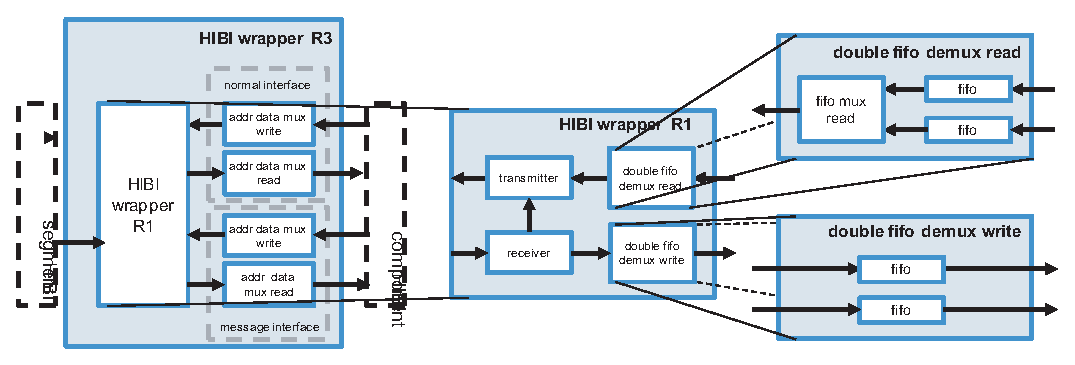
\includegraphics[width=0.9\textwidth]{../Fig/Eps/fig_r3_structure.eps}
    \caption{HIBI R3 wrapper block diagram}
    \label{fig:r3_structure}
  \end{center}
\end{figure*}

\subsection{Resource usage}

The resource usage for invidual HIBI wrappers was acquired from a SoC
that was synthesized to a Arria II GX FPGA on a Arria II GX
development board. The SoC had two HIBI components with both attached
to a R3 HIBI wrapper. The size of the fifos on these wrappers was set
to 4 words which means $4 \cdot 32b = 128 b$ on each fifo. 

Table~\ref{table:resource_usage} shows the combinatorial ALU (adaptive
LUT) counts and register counts of a wrapper. Both minimum and maximum
values are reported since synthesis does not always produce exactly
the same results. Area can be significantly reduced if the FIFOs are
implemented as onchip memories (m9k blocks in Arria II GX).

\begin{table*}
  \caption {Resource usage of wrapper R3, with 32b data, multiplxed address and 5b command.
  \label{table:resource_usage}
    v.2  and v.3 }
  \begin{center}
    \begin{tabular}{l | l | r }
      \hline \hline
      Wrapper subblock & Unit   & Value \\
      \hline \hline
      HIBI wrapper r3 & comb. ALUTs & 724-763 \\
                      & registers   & 1029-1168 \\
      \hline
      HIBI wrapper r1 & comb. ALUTs & 466-533 \\
                      & registers   & 825-935 \\
      \hline
      4-word FIFO     & comb. ALUTs & 76-104 \\
                      & registers   & 155-167 \\                
      \hline
    \end{tabular}
  \end{center}  
\end{table*}


Fig.~\ref{fig_chip_planner} shows the
resource usage layout on the FPGA as seen on the Chip Planner in
Quartus II. The two wrappers are highlighted in blue.


\begin{figure*}
  \begin{center}
    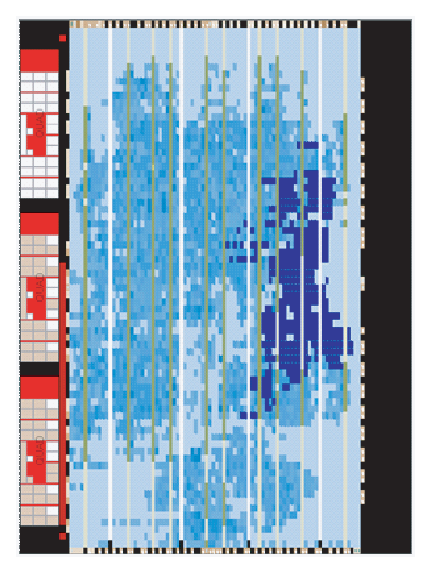
\includegraphics[width=0.4\textwidth]{../Fig/Eps/fig_chip_planner.eps}
    \caption{HIBI R3 in Quartus' chip planner tool}
    \label{fig:chip_plannet}
  \end{center}
\end{figure*}


\subsection{Simulated performance}

The throughput was measured for a 32 bit, 200 MHz HIBI segment with
two components, both of which were connected to the segment with a R3
wrapper. The sender transmitted a continous stream of 1024 words to a
single address. Maximum throughput is $200 MHz \cdot 32b =$ 800
MByte/s. Since the data and address are buses muxed together, the
minimum time to send the stream would be 1025 cycles.  Measured
latency and throughput are shown in Fig.\ref{fig_performance}. Both
approach their theoretical limits as the FIFO depth increases.

\begin{figure*}
  \begin{center}
    \subfigure[Transfer latency in cycles. Theoretical miniumum 1025 cycles (one cycle needed for address)]{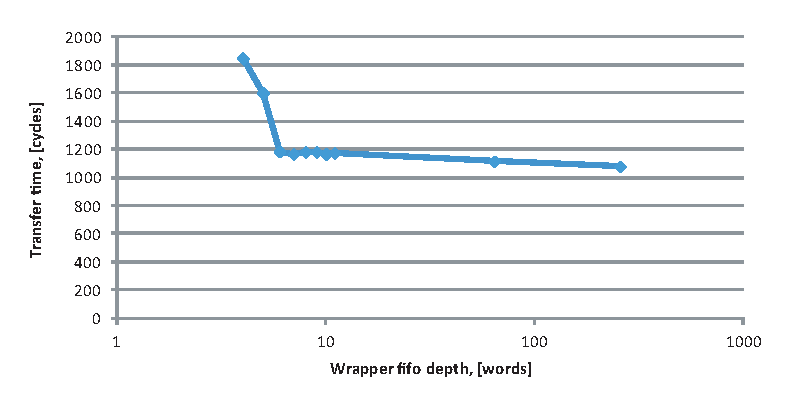
\includegraphics[width=0.85\textwidth]{../Fig/Eps/gra_latency_1024words.eps}
      \label{subfig:perf_latency}}
    \subfigure[Throuhgpput in MB/s. Theoretical max 800 MB/s]{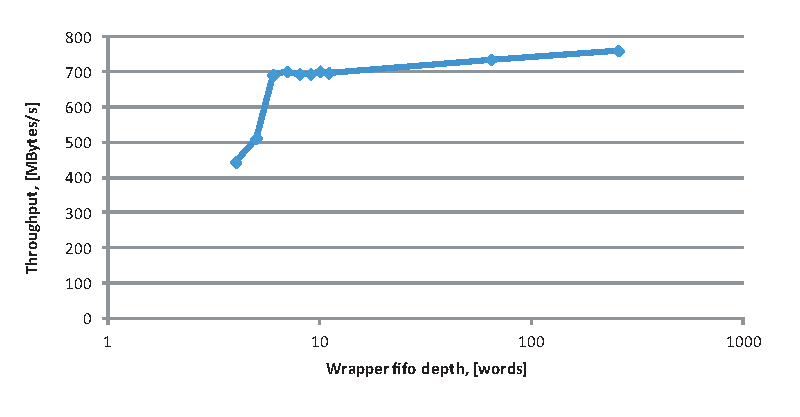
\includegraphics[width=0.85\textwidth]{../Fig/Eps/gra_throughput_1024words.eps}
      \label{subfig:perf_throughput}}
    \caption{Performance with 1024-word transfers.}
    \label{fig:performance}
  \end{center}
\end{figure*}





\section{Usage examples}

IP can connect directly to HIBI but CPUs should use a DMA. It allows
performing transfers on the backgournd while CPU is processing.

\subsection{Transmission with dual-port memory buffer and DMA controller}

Fig.~\ref{fig:dma_tx} shows the concept how CPU can send data using
DMA.
\begin{enumerate}
\item CPU reserves buffer space from dual-port memory
\item CPU copies/writes data to dual-port memory
\item CPU configures DMA transfer: memory address, size of transfer,
  and destination IP-block's HIBI address (not local CPU address)
\item DMA reads data from dual-port memory and sends the data to the
  configured HIBI address
\end{enumerate}


\begin{figure}
  \begin{center}
    {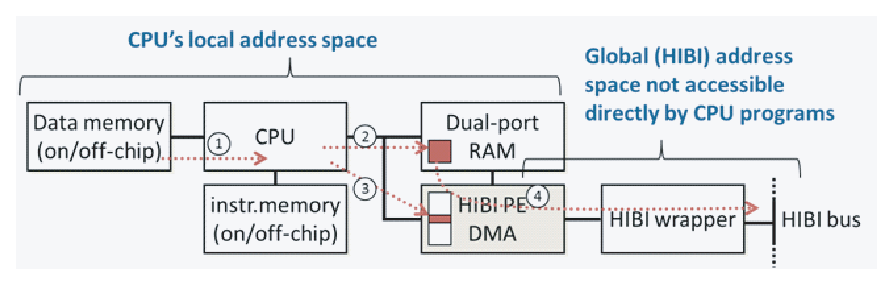
\includegraphics[width=0.7\textwidth]{../Fig/Eps/fig_dma_tx.eps}}
    \caption{Example how CPU sends using DMA.}
    \label{fig:dma_tx}
  \end{center}
\end{figure}


\subsection{Reception with dual-port memory buffer and DMA controller}

Fig.~\ref{fig:dma_rx} shows the concept how CPU can use DMA to copy
received data into the local dual-port memory.

\begin{enumerate}
\item CPU reserves buffer space from dual-port memory
\item CPU configures DMA: Memory address, size of transfer, and the
  HIBI address in which data is received
\item DMA copies the incoming data to DPRAM
\item DMA interrupts CPU when a configured number of words have been
  received
\item CPU knows that data is ready in memory and uses it/copies to
  data memory
\end{enumerate}

\begin{figure}
  \begin{center}
    {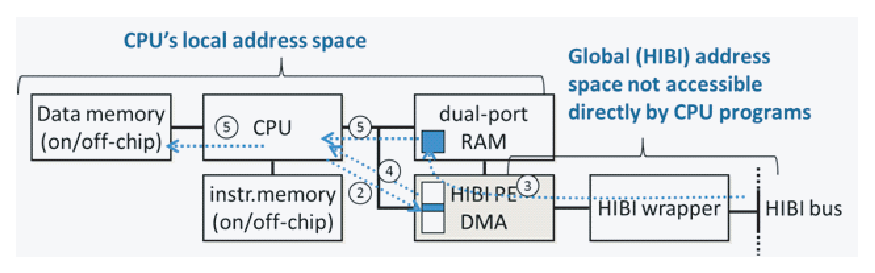
\includegraphics[width=0.7\textwidth]{../Fig/Eps/fig_dma_rx.eps}}
    \caption{Example how CPU receives data usign DMA.}
    \label{fig:dma_rx}
  \end{center}
\end{figure}

Rx buffers are organized as channels. Fig.~\ref{fig:dma_rx_buffers}
shows how DMA translates incoming HIBI addresses into addresses in the
local memory. Only memory space limits how many buffers (channels)
exists at the same time. Channels have implicit meanings that must be
agreed:
\begin{enumerate}

\item Who (what IP-block or CPU) sends data to which channel, since
  otherwise the sender is not known (HIBI does not send sender ID in
  transfers).
\item Possible explicit meaning of channel like ``DCT transform
  Q-parameter''. Then, it is not that relevant who provides data.
\end{enumerate}


\begin{figure}
  \begin{center}
    {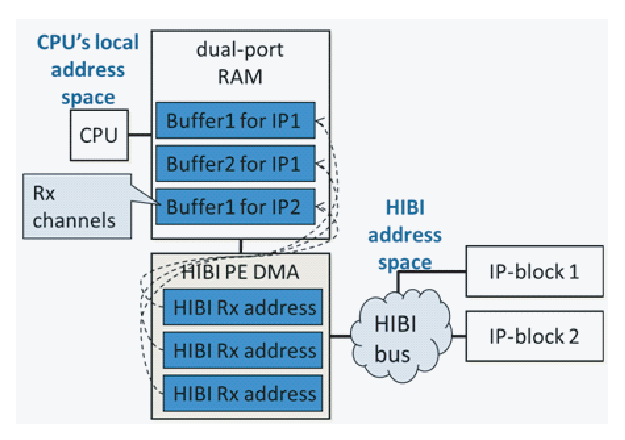
\includegraphics[width=0.5\textwidth]{../Fig/Eps/fig_dma_rx_buffers.eps}}
    \caption{Example mapping between incoming address and buffer in dual-port memory.}
    \label{fig:dma_rx_buffers}
  \end{center}
\end{figure}

\subsection{Example: use source specific addresses}

\begin{figure}
  \begin{center}
    {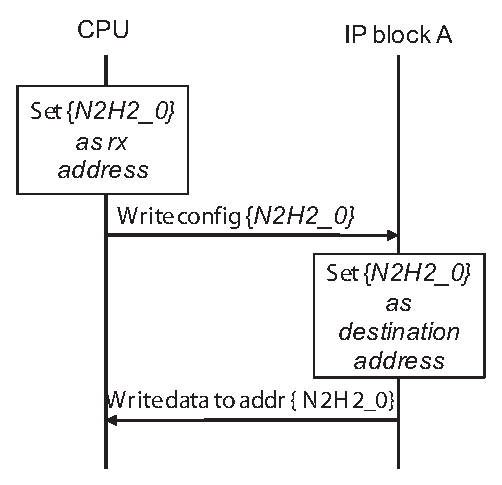
\includegraphics[width=0.5\textwidth]{../Fig/Eps/fig_src_specific_addr.eps}}
    \caption{Example how CPU instructs the IP block where to put result data.}
    \label{fig:src_specific_addr}
  \end{center}
\end{figure}


Designer wished to implement following high-level sequence ``HW
IP-block A should send data to CPU after initialization''. The
procedure to achieve this is
\begin{enumerate}
\item CPU Sets rx buffer address to its DMA block N2H2\_0
\item CPU sends that same address to A's IP-block specific
  configuration register
\item IP A knows now to where send data
\item CPU knows from where data is coming to address
\end{enumerate}

It is assumed that CPU and IP A know the data amount at design
time. Otherwise, it must agreed upon during initialization (that was
omitted for clarity).

\subsection{SW interface to DMA}

There are low-level SW macros available that access the hardware registers
of HIBI PE DMA (abbreaviated as HPD).  They implement a driver, but
can be also used from user programs.

\begin{table*}
  \caption {The SW macros for accessing the DMA controller's registers}
  \label{table:dma_macros}
  \begin{center}
    \begin{tabular}{p{0.5\textwidth} | p{0.5\textwidth} }
      \hline
      Macro & Meaning \\
      \hline \hline

      void HPD\_CHAN\_CONF ( int channel, int mem\_addr, int rx\_addr, int
      amount, int* base ) & Configure HPD channels. After configuration,
      specific channel is ready to receive amount of data to rx\_addr HIBI
      address. Received data is stored to mem\_addr in HPD address space.
      \\
      \hline

      void HPD\_SEND (int mem\_addr, int amount, int haddr, int* base) &
      Send amount of data from mem\_addr to haddr HIBI address. mem\_addr is
      memory address in HPD address space. \\
      \hline
      
      void HPD\_READ (int mem\_addr, int amount, int haddr, int* base) &
      Send command to read amountof data from haddrHIBI address. \\
      \hline
      
      void HPD\_SEND\_MSG (int mem\_addr, int amount, int haddr, int* base)
      & Send amount of data from mem\_addr to haddr HIBI address as HIBI
      message. mem\_addr is memory address in HPD address space.  \\
      \hline
      
      int HPD\_TX\_DONE(int* base) & Returns status of transmit
      operation. \\
      \hline
      
      void HPD\_CLEAR\_IRQ(int chan, int* base) & Clears IRQ of specific
      channel. \\
      \hline
      
      int HPD\_GET\_IRQ\_CHAN(int* base) & Return the number of the channel
      that caused interrupt. If interrupt hasn't occurred, return -1. \\
      \hline
    \end{tabular}
  \end{center}  
\end{table*}

Notes: ``HPD'' is HIBI PE DMA (previously called Nios-to-HIBI 2,
N2H2). ``Base'' is the base address of HIBI PE DMA in HIBI address
space.  ``Amount'' is data amount in 32-bit words.


\begin{table*}
  \caption {The SW functions for using the DMA}
  \label{table:dma_functions}
  \begin{center}
    \begin{tabular}{p{0.5\textwidth} | p{0.5\textwidth} }
      \hline Function & Meaning \\ \hline \hline 

      void HIBI\_TX (uint8* pData, uint32 dataLen, uint32 destAddr,
      uint8 commType) &

      Send data over HIBI. pData is pointer to data, dataLen is length
      of the data in bytes, destAddr is destination HIBI address,
      commType is either HIBI\_TRANSFER\_TYPE\_DATA or
      HIBI\_TRANSFER\_TYPE\_MESSAGE.  Differences to lower level
      macros are the automatic copying of memory to HIBI PE DMA-buffer
      and protection against simultaneous sending in different
      threads.  \\

      \hline

      struct sN2H\_ChannelInfo* N2H\_ReserveChannel( int32 bufferSize,
      void* callbackFunc, bool handleInDsr, bool calledFromDsr, sint32
      channelNum) &

      Reserve a channel for receiving data.  bufferSize Size of the
      data to be received (bytes).  callbackFunc: Function to call
      when the data arrives.  Prototype: function(uint8* pData, uint32
      dataLen, uint32 receivedAddr) handleInDsr: Set to false
      calledFromDsr: Set to false channelNum: Channel that is waiting
      for incoming data. The complete address will be HIBI base
      address + channelNum.  Difference to lower level macros is that
      interrupt handler provided by HIBI driver, own function can be
      registered directly to handle data. \\

      \hline
    \end{tabular}
  \end{center}  
\end{table*}



HIBI\_TX checks that previous send operation is complete and Calls
HPD\_send macro. Hence, it also runs macros HPD\_TX\_ADDR, TX\_AMOUNT, HIBI\_ADDR,
TX\_COMM, and TX\_START Releases the Tx channel.

Following example shows a data transfers between two CPUs assuming the
system in
Fig.~\ref{subfig:dma_example}. Fig.~\ref{subfig:dma_seq_diag} shows
the sequence diagram.


\begin{figure*}
  \begin{center}
    \subfigure[IP sends.]{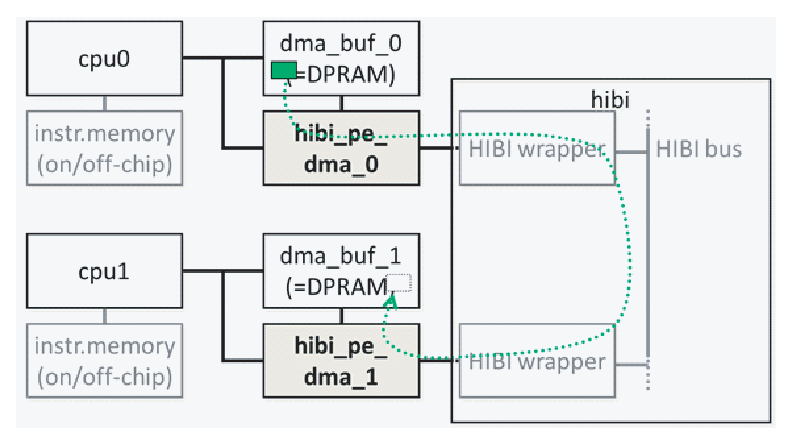
\includegraphics[width=0.85\textwidth]{../Fig/Eps/fig_dma_example.eps}
      \label{subfig:dma_example}}
    \subfigure[IP receives data]{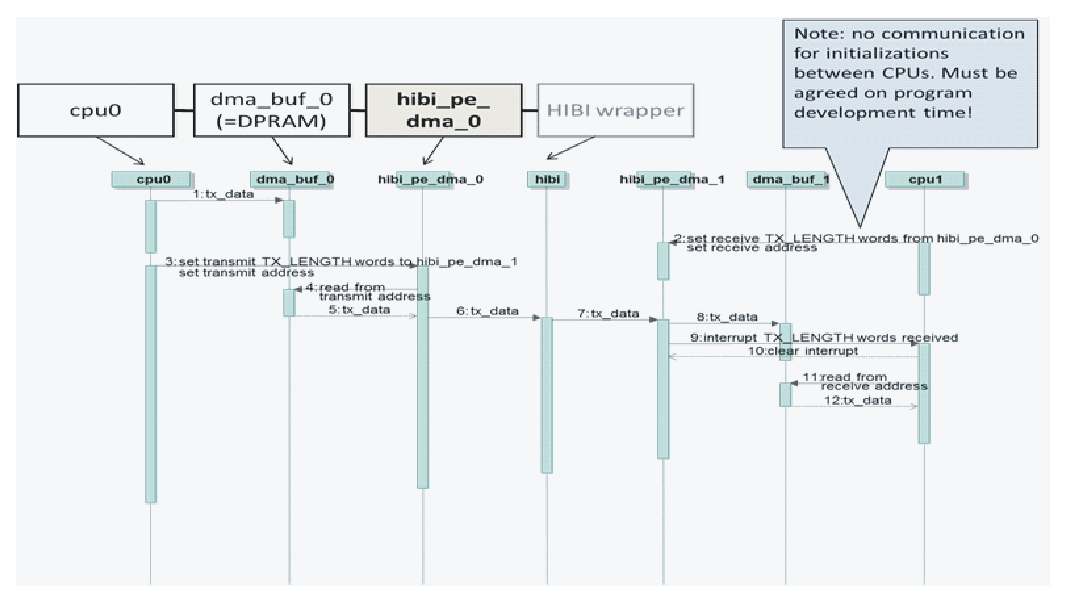
\includegraphics[width=0.85\textwidth]{../Fig/Eps/fig_dma_seq_diag.eps}
      \label{subfig:dma_seq_diag}}
    \caption{Examples of timing at IP interface.}
    \label{fig:dma_example}
  \end{center}
\end{figure*}




\section {Summary}



The most important properties of HIBI are summarized in
Table.~\ref{table:hibi_versions}. HIBI network allows multiple
topologies and utilizes distributed arbitration. The network is
constructed by instantiating multiple wrapper components and and
connecting them together. The wrapper is modular allowing good
parameterization at design time and possibility to reconfigure certain
parameters of the network runtime.
\begin{table*}
  \caption{Properties of HIBI v.3}
  \label{table:hibi_versions}
  \begin{center}
    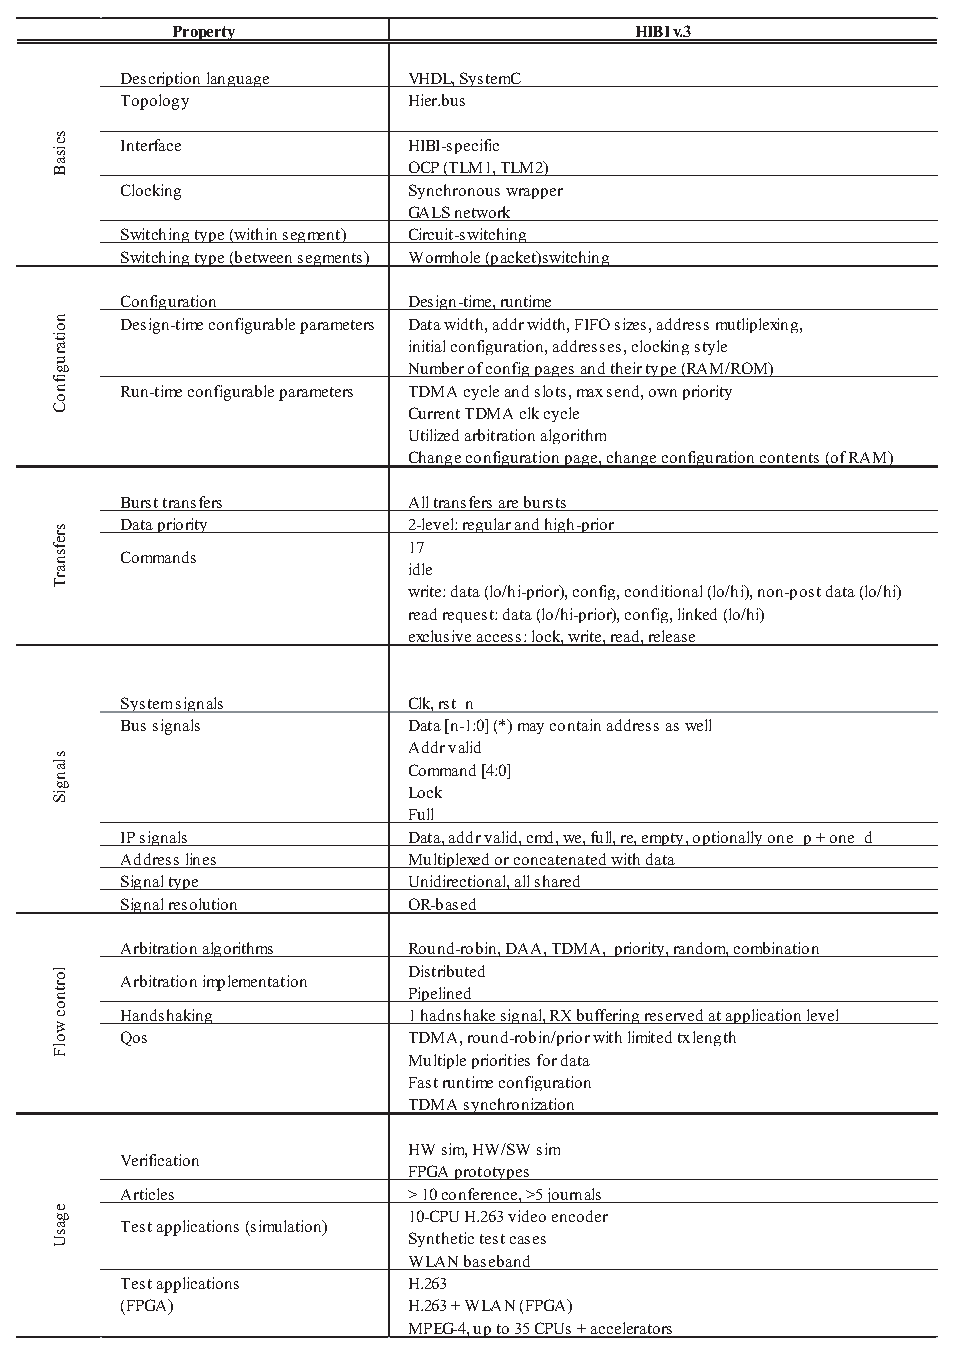
\includegraphics[width=0.9\textwidth]{../Fig/Eps/tab_hibi_v3.eps}
  \end{center}
\end{table*}

\setcounter{secnumdepth}{-1}
\bibliography{IEEEfull,hibi_datasheet_ref}
%\bibliography{hibi_datasheet_ref}
\bibliographystyle{IEEEtranS} 


\end{document}

